\documentclass[reqno]{amsart}
\usepackage[utf8]{inputenc}
\usepackage[margin=1in]{geometry}
\usepackage[usenames, dvipsnames]{xcolor}
\usepackage{graphicx}
\usepackage{mathtools}
\usepackage{amssymb}
\usepackage{amsthm}
\usepackage{fancyhdr}
\usepackage{adforn}
\usepackage{xparse}
\usepackage{tikz}
\usetikzlibrary{fadings}
%\usetikzlibrary{matrix, positioning, calc}
% Additional math macros that I want in both my notes and my psets
\usepackage[sc, noBBpl]{mathpazo}
\usepackage{mathrsfs}
\usepackage[T1]{fontenc}
\usepackage{calligra}
\usepackage{microtype}
\usepackage[all]{xy}
\usepackage{slashed}
\newcommand{\A}{\mathbb A}
\newcommand{\cat}{\mathsf}
\newcommand{\sC}{\cat C}
\newcommand{\sD}{\cat D}
\newcommand{\sS}{\cat S}
\newcommand{\sA}{\mathscr A}
\newcommand{\sF}{\mathscr F}
\newcommand{\sG}{\mathscr G}
\renewcommand{\P}{\mathbb P}
\newcommand{\cO}{\mathscr O}
\newcommand{\sI}{\mathscr I}
\DeclareMathOperator{\coker}{coker}
\renewcommand{\Im}{\operatorname{Im}}
\newcommand{\pt}{\mathrm{pt}}
\DeclareMathOperator{\Hom}{Hom}
\newcommand{\op}{^{\mathsf{op}}}
\newcommand{\Id}{\mathrm{Id}}
\DeclareMathOperator{\Mat}{Mat}
\newcommand{\m}{\mathfrak m}
%\newcommand{\p}{\mathfrak p}
\newcommand{\q}{\mathfrak q}
\DeclareMathOperator{\MSpec}{MSpec}
\DeclareMathOperator{\Spec}{Spec}
\newcommand{\Top}{\cat{Top}}
\newcommand{\Ring}{\cat{Ring}}
\newcommand{\Mod}{\cat{Mod}}
\DeclareMathOperator{\res}{res}
\newcommand{\Alg}{\cat{Alg}}
\newcommand{\Fun}{\cat{Fun}}
\newcommand{\AffSch}{\cat{AffSch}}
\newcommand{\Ab}{\cat{Ab}}
\DeclareMathOperator{\bl}{--}
\DeclareMathOperator{\Free}{Free}
\DeclareMathOperator{\For}{For}
\newcommand{\Set}{\cat{Set}}
\newcommand{\LocRing}{\cat{LocRing}}
\newcommand{\Grp}{\cat{Grp}}
\newcommand{\Sch}{\cat{Sch}}
\newcommand{\inHom}{\operatorname{\underline{\Hom}}}
\DeclareMathOperator{\Frac}{Frac}
\DeclareMathOperator{\Gal}{Gal}
\DeclareMathOperator{\Nil}{Nil}
\newcommand{\pre}{\sC^{\text{pre}}}
\newcommand{\sh}{_{\text{sh}}}
\newcommand{\G}{\mathbb G}
\DeclareMathOperator{\Proj}{Proj}
\newcommand{\sM}{\mathscr M}
\newcommand{\sV}{\mathscr V}
\newcommand{\fU}{\mathfrak U}
\newcommand{\GL}{\mathrm{GL}}
\DeclareMathOperator{\Sym}{Sym}
% http://tex.stackexchange.com/questions/141434/how-to-type-sheaf-hom
\DeclareMathOperator{\shom}{\mathscr{H}\text{\kern -4pt {\calligra\large om}}\,}
\newcommand{\sL}{\mathscr L}
\DeclareMathOperator{\QC}{QC}
\DeclareMathOperator{\Supp}{Supp}
\newcommand{\sN}{\mathscr N}
\DeclareMathOperator{\Ann}{Ann}
\DeclareMathOperator{\Der}{Der}
\newcommand{\ctcpx}[1]{(#1)^{\text{der}}}
\newcommand{\Dist}{\mathsf{Dist}}
\newcommand{\shdi}{\operatorname{Sh}_{\Dist}}
\DeclareMathOperator{\Sh}{Sh}
\newcommand{\shz}{\mathsf{Sh}_{\text{\rm Zar}}}
\DeclareMathOperator{\Gr}{Gr}
% Source: http://tug.org/pipermail/xy-pic/2001-July/000015.html
\newcommand{\pullbackcorner}[1][dr]{\save*!/#1+1.2pc/#1:(1,-1)@^{|-}\restore}
\newcommand{\pushoutcorner}[1][dr]{\save*!/#1-1.2pc/#1:(-1,1)@^{|-}\restore}
\newcommand{\TDel}{\mathrm{2\Delta}}
\DeclareMathOperator{\Bl}{B\ell}
\newcommand{\cR}{\mathcal R}
\newcommand{\cL}{\mathcal L}
\newcommand{\cH}{\mathcal H}
\newcommand{\refR}{\reflectbox{\(\cR\)}}

\renewcommand{\a}{\alpha}
\renewcommand{\b}{\beta}
%\newcommand{\e}{\epsilon}
\renewcommand{\l}{\lambda}
\renewcommand{\L}{\Lambda}
\newcommand{\g}{\gamma}
\newcommand{\s}{\sigma}
\newcommand{\z}{\zeta}
\newcommand{\RR}{\mathbb{R}}
\newcommand{\NN}{\mathbb{N}}
\newcommand{\QQ}{\mathbb{Q}}
\newcommand{\ZZ}{\mathbb{Z}}
\newcommand{\CC}{\mathbb{C}}
\newcommand{\cC}{\mathcal{C}}
\newcommand{\f}{\frac}
\newcommand{\p}{\partial}
\renewcommand{\P}[3][]{\f{\partial^{#1} #2}{\partial #3 ^{#1}}}
%\newcommand{\avg}[1]{\langle #1 \rangle}
\newcommand{\avg}[1]{\left< #1 \right>}
\newcommand{\?}{\overset{?}{=}}
\newcommand{\Int}{\int_{-\infty}^\infty}
\newcommand{\ket}[1]{\left| #1 \right>} % for Dirac bras
\newcommand{\bra}[1]{\left< #1 \right|} % for Dirac kets
\newcommand{\braket}[2]{\left< #1 \vphantom{#2} \right|
 \left. #2 \vphantom{#1} \right>} % for Dirac brackets
\newcommand{\pv}{\vec{p}}

\newcommand{\grad}[1]{\gv{\nabla} #1} % for gradient
\let\divsymb=\div % rename builtin command \div to \divsymb
\renewcommand{\div}[1]{\gv{\nabla} \cdot #1} % for divergence
\newcommand{\curl}[1]{\gv{\nabla} \times #1} % for curl
\renewcommand{\labelenumi}{(\alph{enumi})}
\let\vaccent=\v % rename builtin command \v{} to \vaccent{}
\renewcommand{\v}[1]{\ensuremath{\mathbf{#1}}}
\newcommand{\uv}[1]{\ensuremath{\mathbf{\hat{#1}}}} % for unit vector
\newcommand{\gv}[1]{\ensuremath{\mbox{\boldmath$ #1 $}}} 
% for vectors of Greek letters
\usepackage{hyperref}
\usepackage{siunitx}

%\usepackage[compat=1.1.0]{tikz-feynman}

% TODO fiddle with colors
\definecolor{newblue}{HTML}{1F98A6}
\definecolor{newred}{HTML}{D95448}
\definecolor{neworange}{HTML}{F29441}
\hypersetup{
	colorlinks,
	linkcolor=newred,
	citecolor=neworange,
	urlcolor=newblue!80!black,
}
\usepackage[all]{hypcap}
\pagestyle{plain}
\setcounter{tocdepth}{1}


\usepackage{titlesec}
\titleformat{\section}[frame]
  {\normalfont}
  {\filright
   \footnotesize
   \enspace Lecture \arabic{section}.\enspace}
  {8pt}
  {\Large\bfseries\filcenter}
\usepackage[dotinlabels]{titletoc}
\titlecontents{section}[1.5em]{}{\contentslabel{2.3em}}{\hspace*{-2.3em}}{\hfill\contentspage}

\renewcommand{\sectionmark}[1]{\markleft\thesection. #1}

\fancyhf{}
\fancyhead[RO,LE]{\small\thepage}
\fancyhead[LO]{\small\slshape\nouppercase{\rightmark}}
\fancyhead[RE]{\small\slshape Advanced Quantum Field Theory Lecture Notes}
\setlength{\headheight}{11.0pt}
\pagestyle{fancy}

\numberwithin{equation}{section}
\newcommand{\orbreak}{
\begin{center}
	\adforn{17}\;\(\cdot\)\;\adforn{18}
	\vspace{0.2cm}
\end{center}
}

\renewcommand{\labelitemi}{\(\circ\)}

% I wanted to allow one to reference parts of a thm/cor/etc. and have it print the thm number too, e.g. 29.2(1),
% but this isn't working right now. Probably the best way to do this would be to play around with enumitem to
% define a new enumerate-like counter and then just use that directly instead of enumerate in comp.

% This feels really wobbly, but so far it's working
\NewDocumentEnvironment{comp}{mm}{%
	\csname #1\endcsname\hfill
	\csname #2\endcsname
}{
	\csname end#2\endcsname
	\csname end#1\endcsname
}

% usage:
% \shortexact[f][g]{A}{B}{C},
%
%			 f    g
% for 0 -> A -> B -> C -> 0,
\DeclareDocumentCommand{\shortexact}{O{} O{} mmmm}{
\xymatrix{
	0\ar[r] & #3\ar[r]^-{#1} & #4\ar[r]^-{#2} & #5\ar[r] & 0#6
}}
% exactly the same, but for 0 -> A -> B -> C
\DeclareDocumentCommand{\leftexact}{O{} O{} mmmm}{
\xymatrix{
	0\ar[r] & #3\ar[r]^-{#1} & #4\ar[r]^-{#2} & #5 #6
}}
% ... and the same, for A -> B -> C -> 0
\DeclareDocumentCommand{\rightexact}{O{} O{} mmmm}{
\xymatrix{
	#3\ar[r]^-{#1} & #4\ar[r]^-{#2} & #5\ar[r] & 0#6
}}



% usage:
% X\dblarrow[r] & Y
%   f
% X => Y
%   g
\DeclareDocumentCommand{\dblarrow}{O{} O{} O{}}{
	\ar@<0.4ex>[#1]^-{#2}\ar@<-0.4ex>[#1]_-{#3}
}
% Note: it would be a useful exercise to figure out how to define this so it can be used as
% \dblarrow[r]^f_g

\everyentry={\displaystyle}

\newcommand{\N}{\mathbb N}
\newcommand{\Z}{\mathbb Z}
\newcommand{\Q}{\mathbb Q}
\newcommand{\R}{\mathbb R}
\newcommand{\C}{\mathbb C}
\newcommand{\F}{\mathbb F}
\newcommand{\vp}{\varphi}
\newcommand{\term}{\emph}
\renewcommand{\vec}[1]{\boldsymbol{\mathbf{#1}}}
\DeclarePairedDelimiter\paren{(}{)}
%\DeclarePairedDelimiter\ang{\langle}{\rangle}
\DeclarePairedDelimiter\abs{\lvert}{\rvert}
\DeclarePairedDelimiter\norm{\lVert}{\rVert}
\DeclarePairedDelimiter\bkt{[}{]}
\DeclarePairedDelimiter\set{\{}{\}}
% Swap paren* and paren, etc., so that the normal version resizes by default.
% Meanwhile, one can use \paren*[\Big]{...} to customize the size easily.
% It would be interesting to wrap this up into a custom \definedelimiter command...
\makeatletter
	\let\oldparen\paren
	\def\paren{\@ifstar{\oldparen}{\oldparen*}}
	\let\oldbkt\bkt
	\def\bkt{\@ifstar{\oldbkt}{\oldbkt*}}
\makeatother
\newcommand{\e}{\varepsilon}
\def\qedsymbol{{\small{\ensuremath{\boxtimes}}}}
\newcommand{\inj}{\hookrightarrow}
\newcommand{\surj}{\twoheadrightarrow}
\DeclareMathOperator{\id}{id}
\newcommand{\ud}{\,\mathrm{d}}
\renewcommand{\d}{\mathrm d}
\newcommand{\dfr}[2]{\frac{\mathrm d #1}{\mathrm d #2}}
\newcommand{\pfr}[2]{\frac{\partial #1}{\partial #2}}

%\catcode`\"=13
%\newcommand{"}[1]{^{(#1)}}
\newtheorem{thm}[equation]{Theorem}
\newtheorem*{thm*}{Theorem}
\newtheorem{lem}[equation]{Lemma}
\newtheorem*{lem*}{Lemma}
\newtheorem{cor}[equation]{Corollary}
\newtheorem{prop}[equation]{Proposition}
\newtheorem{obs}[equation]{Observation}
\theoremstyle{definition}
\newtheorem{ex}[equation]{Exercise}
\newtheorem{exm}[equation]{Example}
\newtheorem{defn}[equation]{Definition}
\newtheorem*{claim}{Claim}
\theoremstyle{remark}
\newtheorem*{rem}{Remark}
\newtheorem*{fct}{Fact}
\newtheorem*{note}{Note}

\begin{document}
\title{Quantum Field Theory}
\author{Ian Lim\\ Last updated \today}
\maketitle
{\small\noindent These notes were taken for the \textit{Quantum Field Theory} course taught by Ben Allanach at the University of Cambridge as part of the Mathematical Tripos Part III in Michaelmas Term 2018. I live-\TeX ed them using Overleaf, and as such there may be typos; please send questions, comments, complaints, and corrections to 
\href{mailto:itel2@cam.ac.uk?subject=QFT\%20Lecture\%20Notes}{\texttt{itel2@cam.ac.uk}}.\\
Many thanks to Arun Debray for the {\LaTeX} template for these lecture notes: as of the time of writing, you can find him at \url{https://web.ma.utexas.edu/users/a.debray/}.}

\tableofcontents

\section{Thursday, October 4, 2018}
	\begin{quote}\textit{$2=\pi=i=-1$ in these lectures.} --a former lecturer of Prof. Allanach's.\end{quote}
To begin with, some logistic points. The notes and much of the course material will be based on \href{http://www.damtp.cam.ac.uk/user/tong/qft/qft.pdf}{David Tong's QFT notes} plus some of Prof. Allanach's on cross-sections and decay rates. See \url{http://www.damtp.cam.ac.uk/user/examples/indexP3.html} and in particular \url{http://www.damtp.cam.ac.uk/user/examples/3P1l.pdf} for the notes on cross-sections. In revising these notes, I'll be cross-referencing the Tong QFT notes as well as my copy of Anthony Zee's \textit{Quantum Field Theory in a Nutshell,} which takes a different pedagogical order in starting from the path integral formalism and introducing second quantization (the approach described here) later. Any good education in QFT requires an understanding of both formalisms, and we'll see the path integral next term in \emph{Advanced Quantum Field Theory}.\footnote{Note that the path integral formulation from \emph{Statistical Field Theory}, also taught this term, is precisely equivalent to the path integral that appears in QFT under the identification of one of the Euclidean dimensions of a statistical field theory with the imaginary time dimension of a QFT. This will be more obvious in hindsight.}

After Tuesday's lecture, we'll be assigned one of four course tutors:
\begin{itemize}
    \item Francesco Careschi, fc435@cam.ac.uk
    \item Muntazir Abidi, sma74
    \item Khim Leong, lkw30
    \item Stefano Vergari, sv408
\end{itemize}
Also, the Saturday, November 24th lecture has been moved to 1 PM Monday 26 November, still in MR2. That's it for logistics for now.

\begin{defn}
A \term{quantum field theory} (QFT) is a field theory with an infinite number of degrees of freedom (d.o.f.). Recall that a field is a function defined at all points in space and time (e.g. air temperature is a scalar field in a room wherever there's air). The states in QFT are in general multi-particle states.
\end{defn}
Special relativity tells us that energy can be converted into mass, and so particles are produced and destroyed in interactions (particle number is in general not conserved). This reveals a conflict between SR and quantum mechanics, where particle number is fixed. Interaction forces in our theory then come from additional structure in the theory, depending on things like
\begin{itemize}
    \item symmetry
    \item locality
    \item ``renormalization group flow.''
\end{itemize}

\begin{defn}
A \term{free QFT} is a QFT that has particles but no interactions. The classic free theory is a relativistic theory with which treats particles as excitations of infinitely many quantized harmonic oscillators.
\end{defn}
Free theories are generally not realistic but they are important, as interacting theories can be built from these with perturbation theory. The fact we can do this means the particle interactions are somehow weak (we say these theories have \term{weak coupling}), but other theories of interest (e.g. the strong force) have strong coupling and cannot be described with perturbation theory.

\subsection*{Units in QFT} In QFT, we usually set $c=\hbar=1$. Since $[c]=[L][T]^{-1}$ and $[\hbar]=[L]^2[M][T]^{-1},$ we find that in natural units, $$[L]=[T]=[M]^{-1}=[E]^{-1}$$ (where the last equality follows from $E=mc^2$ with $c=1$, for example). We often just pick one unit, e.g. an energy scale like \si{\electronvolt}, and describe everything else in terms of powers of that unit. To convert back to metres\footnote{As a USAmerican, I am likely to be bewilderingly inconsistent with regards to using American versus British spellings. Please bear with me.} or seconds, just reinsert the relevant powers of $c$ and $\hbar$.

\begin{exm}
The de Broglie wavelength of a particle is given by $\lambda=\hbar/(mc)$. An electron has mass $m_e\simeq \SI{e6}{\electronvolt}$, so $\lambda_e = \SI{2e-12}{\meter}$.
\end{exm}

If a quantity $x$ has dimension $(mass)^d$, we write $[x]=d$, e.g. $$G=\frac{\hbar c}{M_p^2}\implies [G]=-2.$$  $M_p \approx \SI{e19}{\giga\electronvolt}$ corresponds to the Planck scale, $\lambda_p \sim \SI{e-33}{\centi\meter}$, the length/energy scales where we expect quantum gravitational effects to become relevant. We note that the problems associated with relativising the Schr\"odinger equation are fixed in QFT by particle creation and annihilation.

\subsection*{Classical field theory} Before we do QFT, let's review classical field theory. In classical particle mechanics, we have a finite number of generalized coordinates $q_a(t)$ (where $a$ is a label telling you which coordinate you're talking about), and in general they are a function of time $t$. But in field theory, we instead have continuous fields $\phi_a(\vec{x},t)$, where $a$ labels the field in question and $\vec x$ is no longer a coordinate but a label like $a$.\footnote{See for instance Anthony Zee's \textit{QFT in a Nutshell} to see a more detailed description of how we go from discrete to continuous systems.}

In our classical field theory, there are now an infinite number of degrees of freedom, at least one for each position in space $\vec x$, so position has been demoted from a dynamical variable to a mere label.

\begin{exm}
The classical electromagnetic field is a vector field with components $E_i(x,t), B_i(x,t)$ such that $i,j,k\in \{1,2,3\}$ label spatial directions. In fact, these six fields are derived from four fields (or rather four field components), the four-potential $A_\mu(x,t)=(\phi,\vec{A})$ where $\mu\in\{0,1,2,3\}$.

Then the classical fields are simply related to the four-potential by
\begin{equation}
E_i=\P{A_i}{t}-\P{A_0}{x_i} \text{ and } B_i=\frac{1}{2}\epsilon_{ijk} \P{A_k}{x_j}
\end{equation}
with $\epsilon_{ijk}$ the usual \href{https://en.wikipedia.org/wiki/Levi-Civita_symbol}{Levi-Civita symbol}, and where we have used the Einstein summation convention (repeated indices are summed over).
\end{exm}

The dynamics of a field are given by a \term{Lagrangian} $L$, which is simply a function of $\phi_a(x,t), \dot \phi_a(x,t),$ and $\grad \phi_a(x,t)$. This is in precise analogy to the Lagrangian of a discrete system, which is a function of the coordinates $q_a(t)$ and their derivatives $\dot q_a(t)$.
\begin{defn}
We write
\begin{equation}
L=\int d^3 x \mathcal{L}(\phi_a, \p_\mu \phi_a),
\end{equation}
where we call $\mathcal{L}$ the \term{Lagrangian density}, or by a common abuse of terminology simply the Lagrangian.
\end{defn}
\begin{defn}
We may then also define the \term{action}
\begin{equation}
S\equiv \int_{t_0}^{t_1}L dt = \int d^4x \mathcal{L}(\phi_a,\p_\mu \phi_a)
\end{equation}
\end{defn}
Let us also note that in these units we take the action $S$ to be dimensionless, $[S]=0$ (since it appears alone in an exponent, for instance, $e^{iS}$), and so since $[d^4x]=-4$ we have $[\mathcal{L}]=4.$

The dynamical principle of classical field theory is that fields evolve such that $S$ is stationary with respect to variations of the field that don't affect the initial or final values (boundary conditions). That is, $\delta S=0$. A general variation of the fields produces a variation in the action
$$\delta S=\sum_a \int d^4 x\left \{ \P{\mathcal{L}}{\phi_a}\delta\phi_a +\P{\mathcal{L}}{(\p_\mu\phi_a)} \delta(\p_\mu \phi_a)\right\}.$$
Integrating the second term by parts, we find that the variation in the action becomes
$$\delta S= \sum_a \int d^4x \left\{ \P{\mathcal{L}}{\phi_a}\delta \phi_a +\p_\mu \left( \P{\mathcal{L}}{(\p_\mu \phi_a)}\delta \phi_a\right)-\p_\mu \left(\P{\mathcal{L}}{(\p_\mu \phi_a)}\right)\delta \phi_a\right\}.$$

The integral of the total derivative term vanishes for any term that decays at spatial $\infty$ (i.e. $\mathcal{L}$ is reasonably well-behaved) and has $\delta \phi_a(x,t_1)=\delta \phi_a(x,t_0)=0$, as guaranteed by our boundary conditions. Therefore the boundary term goes away and we find that stationary action, $\delta S=0$, implies the \term{Euler-Lagrange equations},
\begin{equation}
\p_\mu\P{\mathcal{L}}{(\p_\mu\phi_a)}-\P{\mathcal{L}}{\phi_a}=0.
\end{equation}

\begin{exm}
Consider the Klein-Gordon field $\phi$, defined as the real-valued field $\phi$ which has a Lagrangian
\begin{equation}
\mathcal{L}=\frac{1}{2} \eta^{\mu\nu}\p_\mu \phi \p_\nu \phi -\frac{1}{2}m^2 \phi^2.
\end{equation}
Here $\eta^{\mu\nu}$ is the standard Minkowski metric\footnote{We use the mostly minus convention here, but honestly the sign conventions are all arbitrary and relativity often uses the other one where time gets the minus sign.}.

To compute the Euler-Lagrange equation for this field theory,
 we see that $$\P{\cL}{\phi}=-m^2\phi \text{ and } \P{\cL}{(\p_\mu \phi)}=\p^\mu \phi.$$
The Euler-Lagrange equations then tell us that $\phi$ obeys the equation of motion $$\p_\mu \p^\mu \phi+m^2\phi = 0,$$ which we call the \emph{Klein-Gordon equation}. It has wave-like solutions $\phi=e^{-ipx}$ with $(-p^2+m^2)\phi=0$ (so that $p^2=m^2$, which is what we expect in units where $c=1$).
\end{exm}

\subsection*{Non-lectured aside: on functional derivatives} If you're like me, you get a little anxious about taking complicated functional derivatives. The easiest way to manage these is to rewrite the Lagrangian so that all terms precisely match the form of the quantity you are taking the derivative with respect to, and remember that matching indices produce delta functions. 

Here's a quick example. To compute $\P{}{(\p_\alpha \phi)}\left[ \p_\mu \phi \p^\mu \phi\right]$, rewrite the term in the brackets as $\eta^{\mu\nu}\p_\mu \phi \p_\nu \phi$ (since we are deriving with respect to a function of the form $\p_\alpha \phi$) and make sure to take the derivative with respect to a new index not already in the expression, e.g. $\p_\alpha \phi$. Then 
\begin{eqnarray*}
\P{}{(\p_\alpha \phi)}\left[ \p_\mu \phi \p^\mu \phi\right]&=&\P{}{(\p_\alpha \phi)}\eta^{\mu\nu}\p_\mu \phi \p_\nu \phi\\
&=& \eta^{\mu\nu} (\delta^\alpha_\mu)\p_\nu \phi + \eta^{\mu\nu} \p_\mu \phi (\delta _\nu^\alpha)\\
&=&2\p^\alpha \phi,
\end{eqnarray*}
where we have raised the index with $\eta^{\mu\nu}$ and written the final expression in terms of $\alpha$ using the delta function. The functional derivative effectively finds all appearances of the denominator exactly as written, including indices up or down, and replaces them with delta functions so the actual indices match. This is especially important in computing the Euler-Lagrange equations for something like Maxwell theory, where one may have to derive by $\p_\mu A_\nu$ and both those indices must match exactly to their corresponding appearances in the Lagrangian.

No one ever taught me exactly how to approach such variational problems, so I wanted to record my strategy here for posterity. It may take a little longer than just recognizing that $\P{}{(\p_\mu \phi)} \frac{1}{2}\p_\nu \phi \p^\nu \phi = \p^\mu \phi$, but this approach always works and it has the benefit of helping avoid careless mistakes like forgetting the factor of $2$ in the example above.
	
\section{Saturday, October 6, 2018}
	Last time, we derived the Euler-Lagrange equations for Lagrangian densities:
\begin{equation}
\p_\mu \P{\mathcal{L}}{(\p_\mu \phi_a)}-\P{\mathcal{L}}{\phi_a}=0.
\end{equation}
Today, we'll look at some more simple Lagrangians. We'll introduce Noether's theorem as it applies to fields and also derive the energy-momentum tensor in a field theory context.

\begin{exm}
Consider the Maxwell Lagrangian,
\begin{equation}
\mathcal{L}=-\frac{1}{2}(\p_\mu A_\nu)(\p^\mu A^\nu)+\frac{1}{2}(\p_\mu A^\mu)^2.
\end{equation}
Plugging into the E-L equations, we find that $\P{\cL}{A_\nu}=0$ and
\begin{equation}
\P{\cL}{(\p_\mu A_\nu)}=\p^\mu A^\nu +\eta^{\mu\nu}\p_\rho A^\rho.
\end{equation}
Thus E-L tells us that
\begin{equation}
0=-\p^2 A^\nu+\p^\nu (\p_\rho A^\rho)=-\p_\mu(\p^\mu A^\nu-\p^\nu A^\mu).
\end{equation}
Defining the field strength tensor $F^{\mu\nu}=\p^\mu A^\nu-\p^\nu A^\mu$, we can write the E-L equation for Maxwell as the simple
$$0=\p_\mu F^{\mu\nu},$$
which written explicitly is equivalent to Maxwell's equations in vacuum (we'll revisit this when we do QED).
\end{exm}

The Lagrangians we'll consider here and afterwards are all \term{local}-- in other words, there are no couplings $\phi(\vec{x},t)\phi(\vec{y},t)$ with $\vec{x}\neq \vec{y}$. There's no reason a priori that our Lagrangians have to take this form, but all physical Lagrangians seem to do so.

\subsection*{Lorentz invariance} Consider the Lorentz transformation on a scalar field $\phi(x)\equiv \phi (x^\mu)$. The coordinates $x$ transform as $x'=\Lambda^{-1} x$ with $\Lambda^\mu{}_\sigma \eta^{\sigma\tau}\Lambda^\nu{}_\tau = \eta^{\mu\nu}$. Under $\Lambda,$ our field transforms as $\phi\to \phi'$ where $\phi'(x)=\phi(x')$. Recall that Lorentz transformations generically include boosts as well as rotations in $\RR^3$. As we've discussed in Symmetries, Fields and Particles, Lorentz transformations form a Lie group ($O(3,1)$, or specifically the proper orthochronous Lorentz group) under matrix multipication. They have a representation given on the fields (i.e. a mapping to a set of transformations on the fields which respects the group multiplication law).

For a scalar field, this is $\phi(x)\to \phi(\Lambda^{-1}x)$ (an active transformation). We could have also used a passive transformation where we re-label spacetime points: $\phi(x)\to \phi(\Lambda x)$. It doesn't matter too much-- since Lorentz transformations form a group, if $\Lambda$ is a Lorentz transformation, so is $\Lambda^{-1}$. In addition, most of our theories will be well-behaved and Lorentz invariant.

\begin{defn}
\term{Lorentz invariant} theories are ones where the action $S$ is unchanged by Lorentz transformations.
\end{defn}

\begin{exm}
Consider the action given by
$$S=\int d^4x \left[\frac{1}{2} \p_\mu \phi \p^\mu \phi-U(\phi)\right],$$
where $U(\phi)$ is some potential density. $U\to U'(x) \equiv U(\phi'(x))= U(x')$ means that $U$ is a scalar field (check this!) and we see that
$$\p_\mu \phi' =\P{}{{x^\mu}}\phi(x')=\P{{{x'}^\sigma}}{{x^\mu}} \p_\sigma' \phi(x')= (\Lambda^{-1})^\sigma{}_\mu \p_\sigma' \phi(x')$$
where $\p_\sigma' \equiv \P{}{{{x'}^\sigma}}$.
Thus the kinetic term transforms as
$$\cL_{kin} \to \cL_{kin}'=\eta^{\mu\nu}\p_\mu \phi' \p_\nu \phi' =\eta^{\mu\nu}(\Lambda^{-1})^\sigma{}_\mu (\Lambda^{-1})^\tau{}_\nu \p_\sigma' \phi(x') \p_\tau' \phi(x')=\eta^{\sigma\tau} \p_\sigma' \phi(x')\p_\tau' \phi(x') = L_{kin}(x).$$

Thus we see that the action overall transforms as
$$S\to S' = \int d^4 x \cL(x')=\int d^4 x \cL(\Lambda^{-1}x).$$
Under a change of variables $u \equiv \Lambda^{-1} x$, we see that $\det(\Lambda^{-1})=1$ (from group theory) so the volume element is the same, $d^4y=d^4x$ and therefore
$$S'=\int d^4 y\, \cL(y)=S.$$
We conclude that $S$ is invariant under Lorentz transformations.
\end{exm}

We also remark that under a LT, a vector field $A_\mu$ transforms like $\p_\mu \phi$, so $$A_\mu'(x) = (\Lambda^{-1})^\sigma{}_\mu A_\sigma (\Lambda^{-1}x).$$
This is enough to attempt Q1 from example sheet 1.\footnote{Copied here for quick reference: Show directly that if $\phi(x)$ satisfies the Klein-Gordon equation, then $\phi(\Lambda^{-1} x)$ also satisfies this equation for any Lorentz transformation $\Lambda.$}

\begin{thm}
Every continuous symmetry of $\cL$ gives rise to a current $J^\mu$ which is conserved, $\p_\mu j^\mu=0$. Each $j^\mu$ has a conserved charge $Q=\int_{\RR^3} j^0 d^3x$.
\end{thm}
Given that the current is conserved, it's easy to show that the charge is conserved, since $\frac{dQ}{dt}=\int_{\RR^3} d^3x \p_0 j^0  = -\int_{\RR^3} d^3 x \div {\vec{j}} =0$ by the divergence theorem, assuming $|\vec{j}|\to 0$ as $|\vec{x}|\to \infty$.

Let us define an infinitesimal variation of a field $\phi$,
$\phi(x)\to \phi'(x)=\phi(x)+\alpha \Delta \phi(x)$
with $\alpha$ an infinitesimal change. If $S$ is invariant, we call this a \term{symmetry} of the theory.

Since $S$ is invariant up to adding a total 4-divergence (a total derivative $\p_\mu$) to the Lagrangian, our symmetry doesn't affect the Euler-Lagrange equations. $\cL$ transforms as
\begin{equation}\label{lagrangeinfinitesimal}
    \cL(x)\to \cL(x)+\alpha \p_\mu X^\mu(x),
\end{equation}
and expanding to leading order in $\alpha$ we have
\begin{equation}
    \cL\to \cL(x)+\alpha \P{\cL}{\phi}\Delta \phi +\alpha \P{\cL}{(\p_\mu\phi)}\p_\mu(\Delta\phi)+O(\alpha^2).
\end{equation}
We can rewrite this in terms of a total derivative $\p_\mu\left(\P{\cL}{(\p_\mu\phi)}\Delta \phi\right)$
so that
\begin{equation}
\cL'=\cL(x)+\alpha \p_\mu\left(\P{\cL}{(\p_\mu\phi)}\Delta \phi\right) +\alpha \left(\P{\cL}{\phi}-\p_\mu \P{\cL}{(\p_\mu\phi)}\right)\Delta \phi.
\end{equation}
By Euler-Lagrange, the second term in parentheses vanishes, so we identify the first term in parentheses as none other than $\alpha \p_\mu X^\mu(x)$ from Eqn. \ref{lagrangeinfinitesimal} (in other words, $\p_\mu\left(\P{L}{(\p_\mu\phi)}\Delta \phi\right) =\p_\mu X^\mu$) and recognize 
\begin{equation}
j^\mu\equiv\P{L}{(\p_\mu \phi)}\Delta \phi -X^\mu
\end{equation} as our conserved current (such that $\p_\mu j^\mu =0$).

\begin{exm}
Take a complex scalar field $$\psi(x)=\frac{1}{\sqrt{2}}(\phi_1(x)+i\phi_2(x)).$$ We can then treat $\psi, \psi^*$ as independent variables and write a Lagrangian
$$L=\p_\mu \psi^* \p^\mu \psi - V(|\psi|^2).$$
Then we observe that under $\psi\to e^{i\beta}\psi, \psi^* \to e^{-i\beta}\psi^*,$ the Lagrangian is invariant. The differential changes are $\Delta \psi = i \psi$ (think of expanding $\psi\ \to e^{i\beta}\psi$ to leading order) and similarly $\Delta \psi^*=-i\psi^*$ (here we find that $X^\mu=0$).

We add the currents from $\psi, \psi^*$ to find
$$j^\mu = i\set{ \psi \p_\mu \psi^* - \psi^* \p_\mu \psi}.$$
\end{exm}
This is enough to do questions 2 and 3 on the example sheet.
\begin{exm}
Under infinitesimal translation $x^\mu \to x^\mu -\alpha \epsilon^\mu$, we have $\phi(x)\to \phi(x)+\alpha \epsilon^\mu \p_\mu \phi(x)$ by Taylor expansion (similar for $\p_\mu\phi$). If the Lagrangian doesn't depend explicitly on $x$, then $\cL(x)\to \cL(x) +\alpha \epsilon^\mu \p_\mu \cL(x)$.

Rewriting to match the form $\cL+\a \p_\mu X^\mu$, we see that our new Lagrangian takes the form
$L(x)+\alpha \epsilon^\nu \p_\mu (\delta^\mu_\nu L)$. We get one conserved current for each component of $\epsilon^\nu$, so that
$$(j^\mu)_\nu = \P{\cL}{(\p_\mu \phi)}\p_\nu \phi - \delta^\mu_\nu \cL$$ with $\p_\mu(j^\mu)_\nu=0$.
We write this as $j^\mu{}_\nu \equiv T^\mu{}_\nu$, the energy-momentum tensor. 

\begin{defn}
The \term{energy-momentum tensor} (sometimes \term{stress-energy tensor}) is the conserved current corresponding to translations in time and space. It takes the form 
$$T^{\mu\nu} \equiv \P{\cL}{(\p_\mu \phi)}\p^\nu \phi - \eta^{\mu\nu} \cL,$$
where we have raised an index with the Minkowski metric as is conventional. The conserved charges from integrating $\int d^3x T^{0\nu}$ end up being the total energy $E=\int d^3x T^{00}$ and the three components of momentum $P^i=\int d^3x T^{0i}$.\footnote{The definition of the energy-momentum tensor here is slightly different from the one used in general relativity. Here, we have used time and space translations to derive $T^{\mu\nu}$, but in general relativity, we use variations of the metric $g^{\mu\nu}$ instead. The benefit of the GR definition is that the resulting tensor is always symmetric, whereas the $T^{\mu\nu}$ from spacetime translations is not guaranteed to be symmetric. We'll see an example of this in the example sheets, but the $T^{\mu\nu}$ defined by spacetime translations can always be \emph{made} symmetric by defining the ``Belinfante-Rosenfeld tensor.'' The construction isn't anything too special, but relativists insist that variations of the action with respect to the metric is the correct way to define the energy-momentum tensor.}
\end{defn}
\end{exm}
	
\section{Tuesday, October 9, 2018}
	Having introduced the matrix groups, we'll next discuss some important subgroups of $GL(n,\RR)$. First, the \term{orthogonal groups.}
\begin{defn}
Orthogonal groups $O(n)$ are the matrix groups which preserve the Euclidean inner product,
\begin{equation}
O(n)=\set{M\in GL(n,\RR): M^T M = I_N}.
\end{equation}
Their elements correspond to orthogonal transformations, so that for $\vec{v}\in \RR^n$, an orthogonal matrix $M$ acts on $\vec{v}$ by matrix multiplication,
$$\vec{v}'=M\cdot \vec{v}$$
and so in particular
$$|\vec{v}'|^2={\vec{v}'}^T \cdot \vec{v}' = \vec{v}^T \cdot M^T M \cdot \vec{v}= \vec{v}^T \cdot \vec{v}=|\vec{v}|^2.$$
It also follows that $\forall M\in O(n), \det(M^TM)=\det(M)^2 = \det(I_n) = 1 \implies \det M =\pm 1$.
\end{defn}
$\det M$ is a smooth function of the coordinates, but our constraint equation means that $\det M$ can only take on one of two discrete values. The orthogonal group $O(n)$ has therefore two connected components corresponding to $\det M = +1$ and $\det M = -1$. The connected component containing the origin ($\det M = +1$) is the special orthogonal group $SO(n)$.
\begin{defn}
The \term{special orthogonal groups} $SO(n)$ are the subset of orthogonal groups which also preserve orientation (i.e. no reflections):
$$SO(n)\equiv \set{M\in O(n): \det M = +1}.$$
That is, elements of $SO(n)$ preserve the sign of the volume element in $\RR^n$,
$$\Omega= \epsilon^{i_1 i_2 \ldots i_n} v_1^{i_1}v_2^{i_2}\ldots v_n^{i_n}.$$
\end{defn}
In contrast, $O(n)$ matrices may include reflections as well as rotations when $\det M = -1$.

\begin{ex}\label{groupaxiomsson}
Check the group axioms for $SO(n)$.\footnote{As usual, we need to check closure and inverses. The identity matrix $I$ satisfies $I^TI=I$ and $\det I=1$, and associativity follows from standard matrix multiplication. Inverses: if $M\in SO(n)$, then $M^{-1}$ is defined by $MM^{-1}=I$. But $\det(MM^{-1})=\det(M)\det(M^{-1})=(1)\det(M^{-1})=\det I = 1$, so $\det(M^{-1})=1$. We also check that the inverse of an orthogonal matrix is also orthogonal: $M M^{-1}=I$, so $(M^{-1})^T (M^T)= (M^{-1})^T M^{-1} =I^T = I$. Closure: $\forall M,N \in SO(n), \det(MN)=\det(M)\det(N)=(1)(1)=1$ and $(MN)^T(MN)=N^TM^T M N= I$, so $MN\in SO(n)$. \qed}
Show that $\dim(O(n))=\dim(SO(n))=\frac{1}{2} n(n-1)$.\footnote{This can be seen by writing a matrix $M\in SO(n)$ as a row of $n$ column vectors $(\vec{x_1},\vec{x_2},\ldots,\vec{x_n})$. Then the condition that $M^T M = 1$ is equivalent to
$\begin{pmatrix}
\vec{x_1}\cdot \vec{x_1} & \vec{x_1}\cdot \vec{x_2} & \ldots &\vec{x_1}\cdot \vec{x_n}\\
\vec{x_2}\cdot \vec{x_1} & \vec{x_2}\cdot \vec{x_2} & \ldots &\vec{x_2}\cdot \vec{x_n}\\
\vdots\\
\vec{x_n}\cdot \vec{x_1}& \ldots & \ldots & \vec{x_n} \cdot \vec{x_n}
\end{pmatrix}= I_n.$
We see that by the symmetry of the explicit form of $M^T M$, we get $1+2+3+\ldots+n = n(n+1)/2$ independent constraints on the $n^2$ entries of $M$. Applying our theorem, we find that the resulting manifold has dimension $n^2-n(n+1)/2=n(n-1)/2$.
} 
\end{ex}

Orthogonal matrices have some nice properties. Let $M \in O(n)$ be an orthogonal matrix and suppose that $\vec{v}_\lambda$ is an eigenvector of $M$ with eigenvalue $\lambda.$ Then the following is true:
\begin{enumerate}
\item If $\lambda$ is an eigenvalue, then $\lambda^*$ is also an eigenvalue (eigenvalues of $M$ come in complex conjugate pairs).
\item $|\lambda|^2=1$.
\end{enumerate}
The proof is as follows:
\begin{enumerate}
\item $M\cdot \vec{v}_\lambda = \lambda \vec{v}_\lambda \implies M\cdot \vec{v}_\lambda^* = \lambda^* \vec{v}_\lambda^*$ (since $M$ is a real matrix).\footnote{This is generally true of real matrices with complex eigenvalues-- it's not specific to orthogonal matrices.}
\item For any complex vector $\vec{v}$, we have
$$(M\cdot \vec{v}^*)^T \cdot M \cdot \vec{v} = \vec{v}^\dagger \cdot M^T M \cdot \vec{v} = \vec{v}^\dagger \cdot \vec{v}.$$ Now if $\vec{v}=\vec{v}_\lambda$, then
$$(M\cdot \vec{v}_\lambda^*)^T \cdot M \cdot \vec{v}_\lambda=(\lambda^* \vec{v}^*_\lambda)^T \cdot (\lambda \vec{v}_\lambda)=|\lambda|^2 \vec{v}_\lambda^\dagger \cdot \vec{v}_\lambda.$$
By comparison to the first expression, we see that $|\lambda|^2=1$. \qed
\end{enumerate}

\begin{exm}
For the group $G=SO(2)$, $M\in SO(2)\implies M$ has eigenvalues
$$\lambda=e^{i\theta},e^{-i\theta}$$ for some $\theta\in\RR,\theta \sim \theta+2\pi$ (identified up to a phase of $2\pi$). A group element may be written explicitly as
$$M=M(\theta)=\begin{pmatrix}
\cos\theta & -\sin\theta\\
\sin\theta & \cos\theta
\end{pmatrix},$$
which is uniquely specified by a rotation angle $\theta$. Therefore the group manifold of $SO(2)$ is $M(SO(2))\cong S^1$, the circle, and we see that $SO(2)$ is an abelian group..

It's not too hard to check using the trig addition formulas that the matrices $M$ written this way really do form a representation of $SO(2)$, since $M(\theta_1) M(\theta_2)=M(\theta_1+\theta_1)$.
\end{exm}
\begin{exm}
For the group $G=SO(3)$, we have instead $M\in SO(3)\implies M$ has eigenvalues
$$\lambda=e^{i\theta},e^{-i\theta},1$$ for $\theta\in \RR,\theta \sim \theta+2\pi$, using our two properties again of paired eigenvalues and modulus 1.
The normalized eigenvector for $\lambda=1$, $\uv n \in \RR^3$, specifies the axis of rotation ($M \cdot \uv n = \uv n$ and $\uv n \cdot \uv n = 0$).

A general group element of $SO(3)$ can be written explicitly as
\begin{equation}
M(\uv n, \theta)_{ij} = \cos\theta\delta_{ij} +(1-\cos\theta)n_i n_j - \sin\theta \epsilon_{ijk} n_k.
\end{equation}
Let us remark that our group is invariant under the identification $\theta\to 2\pi-\theta, \uv n \to -\uv n$. It's also true that we should identify all $M$ with $\theta=0$ since $M(\uv n, 0)= I_3 \forall \uv n$.

We also observe that we can consider the vector
$$\vec{w}\equiv\theta \uv n$$ which lives in the region
$$B_3=\set{\vec{w}\in \RR^3: |\vec w|\leq \pi} \subset \RR^3$$
with boundary
$$\partial B_3 = \set{\vec{w}\in \RR^3: |\vec{w}|=\pi} \cong S^2.$$
We say that the group manifold $M(SO(3))$ then comes from identifying antipodal points on $\p B_3$ ($\vec{w} \sim -\vec{w} \forall \vec{w} \in \p B_3$). See Fig. \ref{so3manifold} for an illustration.
\end{exm}

\begin{figure}\label{so3manifold}
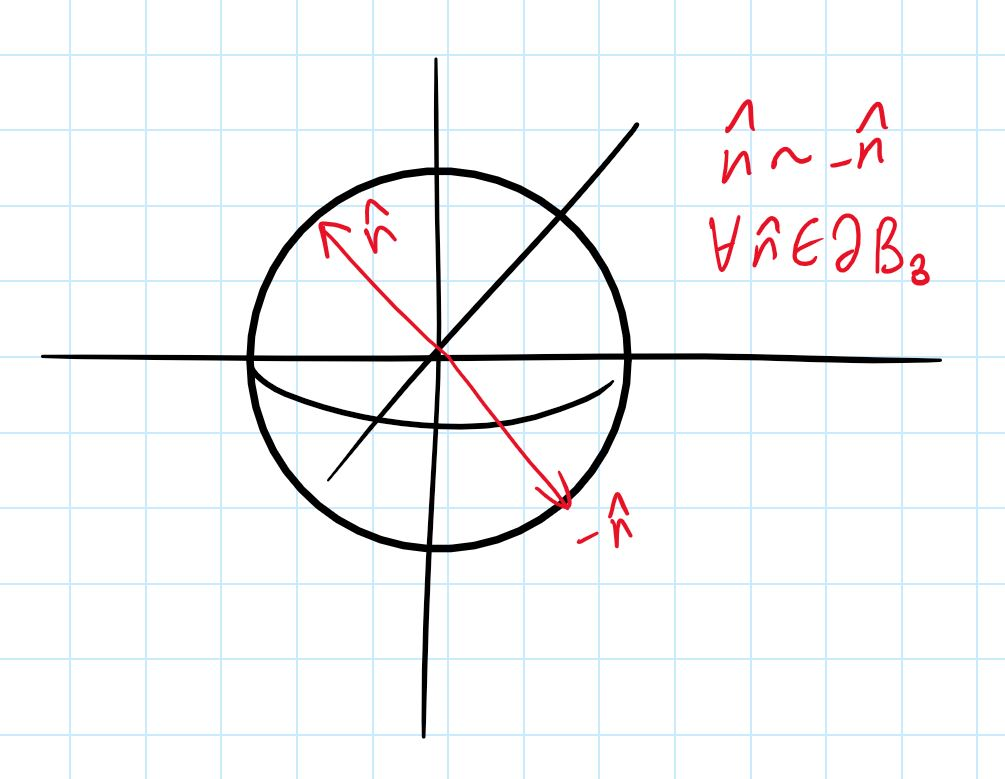
\includegraphics[scale=0.7]{2018/10/20181009_img1}
\caption{The group manifold $M(SO(3))$ is isomorphic to the 3-ball $B^3$ with antipodal points on the boundary identified, $\vec{w} \sim -\vec{w} \forall \vec{w} \in \p B_3$.}
\end{figure}

\begin{defn}
A \term{compact} set is any bounded, closed set in $\RR^n$ with $n\geq 0$. For instance, the $2$-sphere $S^2$ is clearly bounded in $\RR^3$. But the hyperboloid $H^2$ (embedded in $\RR^3$ as $x^2+y^2-z^2 =r^2$) is not bounded, since for any distance $r_0$ one can construct a point $\vec{x}$ on $H^2$ which has $|\vec{x}|>r_0$.
\end{defn}

Let us note some properties of the group manifold $M(SO(3))$. It is compact and connected, but it is not simply connected.
\begin{defn}
A space is \term{simply connected} if all loops on the space are contractible (in the language of algebraic topology, its fundamental group $\pi_1$ is trivial).
\end{defn}
A bit of intuition for why $M(SO(3))$ is topologically non-trivial: draw a path to the boundary, come out on the antipodal side, and go back to the origin. As it turns out, this is different from $S^1$ or the torus $T^2$: whereas these have the full $\ZZ$ as (part of) their fundamental groups ($T^2$ is simply $S^1\times S^1$), if we go around twice in $SO(3)$ we find that this new loop is actually a trivial loop (see Fig. \ref{z2inso3}). Therefore the fundamental group of $SO(3)$ is not infinite but the cyclic group $\ZZ_2$ (i.e. the set $\set{0,1}$ under the group operation $+\mod 2$).

\begin{figure}\label{z2inso3}
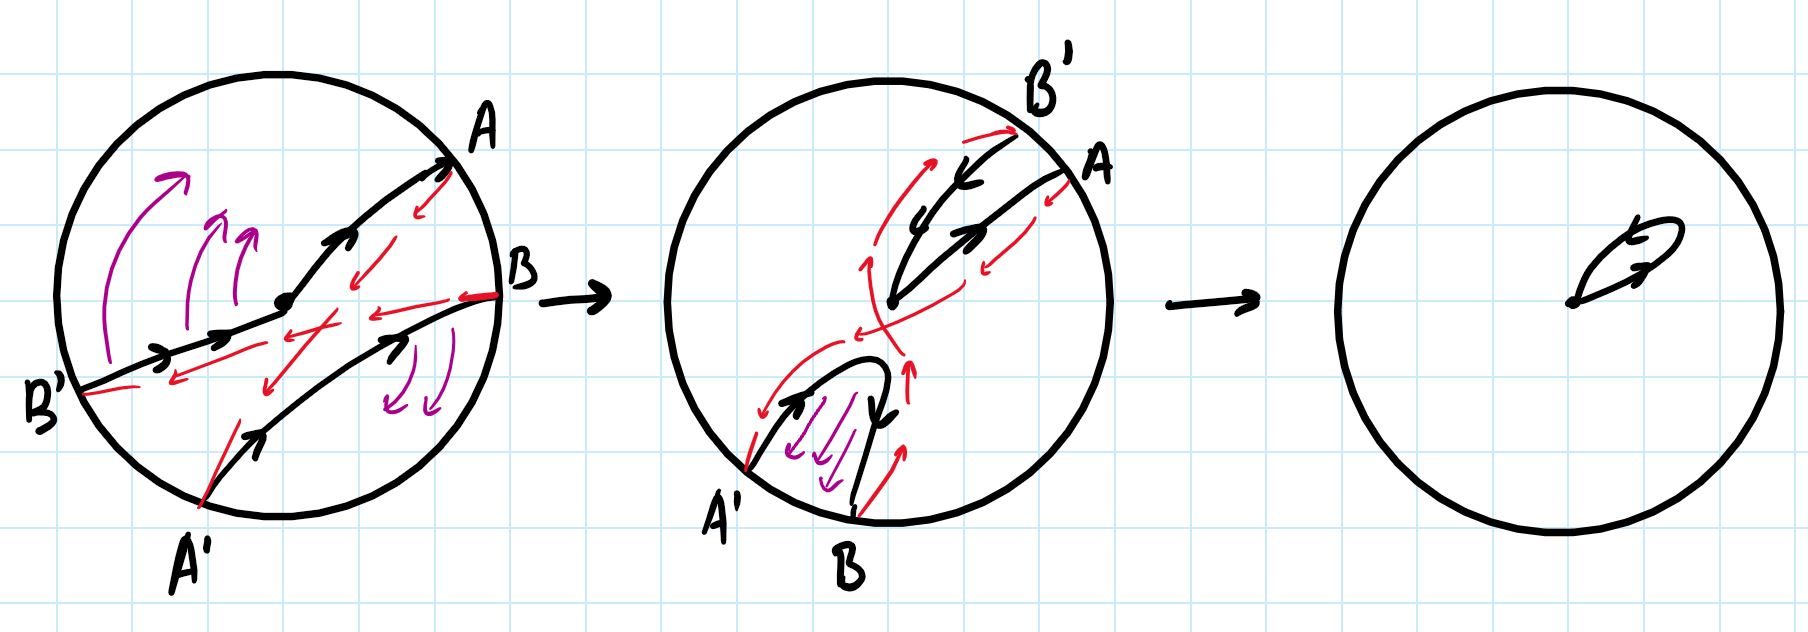
\includegraphics[scale=0.6]{2018/10/20181009_img2}
\caption{A sketch of why the loop which goes through the boundary $\p B_3$ twice is homotopic to (can be continuously deformed into) the trivial loop. For simplicity, consider a circular cross-section of $B_3$ and suppose the loop passes through the boundary at points $A$ ($\sim A'$) and $B$ ($\sim B'$). As we continuously move the point $B$ to $A'$, $B'$ must also move towards $A$, as we see in the second image. We then pull the bit of loop from $A'$ to $B$ through the boundary and find that the resulting loop is trivial (sketch 3). Solid black lines indicate the actual loop path, red dashed arrows indicate the effect of identifying antipodal points, and purple arrows suggest the direction of loop deformation between each drawing.}
\end{figure}
	
\section{Thursday, October 11, 2018}
	Recall that for a free scalar field $$\phi(\vec{x},t)=\int \frac{d^3 \vec{p}}{(2\pi)^3} e^{i \vec{p}\cdot \vec{x}}\phi(\vec{p},t),$$ where
$$\left[\P[2]{}{t}+(\vec{p}^2 +m^2)\right]\phi(\vec{p},t)=0.$$
We also defined $\omega_{\vec{p}}^2\equiv \vec{p}^2 +m^2$.
Our theory has plane wave solutions. 
Let's apply the simple harmonic oscillator quantization process to free fields now, defining
$$\phi(\vec{x})=\int \frac{d^3 \vec{p}}{(2\pi)^3}\frac{1}{\sqrt{2\omega_{\vec p}}}(a_{\vec p}e^{i\vec{p} \cdot \vec x}+a^\dagger_{\vec p}e^{-i\vec{p} \cdot \vec x}).$$
We also have the related conjugate momentum to the field,
$$\pi(\vec{x})=\int \frac{d^3 \vec{p}}{(2\pi)^3}(-i)\sqrt{\frac{\omega_{\vec p}}{2}}(a_{\vec p}e^{i\vec{p} \cdot \vec x}-a^\dagger_{\vec p}e^{-i\vec{p} \cdot \vec x}).$$

In the \term{second quantization} process, we've written our infinite number of harmonic oscillators in momentum space. We want to impose the equivalent of $$[a_{\vec p},a_{\vec q}]=[a^\dagger_{\vec p}, a^\dagger_{\vec q}]=0$$ and $$[a_{\vec p}, a_{\vec q}^\dagger]=(2\pi)^3 \delta^3(\vec p -\vec q).$$

Thus in the field theory context we have instead
$$[\phi(\vec x), \phi(\vec y)]= [\pi (\vec x), \pi (\vec y)]=0$$
and
$$[\phi(\vec x), \pi (\vec y)]=i\delta^3 (\vec x - \vec y).$$

It's a good exercise to check this, but we can for instance check this one way: assume the $a, a^\dagger$ commutation relations:
$$[\phi(\vec x),\pi(\vec y)]=\int \frac{d^3 \vec p}{(2\pi)^3} \frac{d^3 \vec q}{(2\pi)^3} \frac{(-1)}{2}\sqrt{\frac{\omega_{\vec q}}{\omega_{\vec p}}}\set{ -[a_{\vec p}, a_{\vec q}^\dagger] e^{i\vec p \cdot \vec x - i\vec q \cdot \vec y}+[a_{\vec p}^\dagger, a_{\vec q}] e^{-i\vec p \cdot \vec x + i\vec q \cdot \vec y}}.$$
Using these commutation relations, we can rewrite and do the integral over $\vec q$ to get a delta function setting $\vec p = \vec q$,
$$\int \frac{d^3 \vec p}{(2\pi)^3}\left(\frac{-i}{2}\right)\set{-e^{i\vec p \cdot (\vec x - \vec y)}-e^{-i\vec p \cdot (\vec x - \vec y)}=i \delta^3 (\vec x - \vec y)}$$
since $\delta^3(\vec x)= \int \frac{d^3 \vec p}{(2\pi)^3} e^{i \vec p \cdot \vec x}$.

Now we compute $H$ in terms of $a_{\vec p} a_{\vec p}^\dagger$ to find (after some work with $\delta$ functions which you should check) that
\begin{eqnarray*}
H&=&\frac{1}{2}\int d^3 x \left( \pi^2+(\grad \phi)^2+m^2\phi^2\right)\\
&=& \frac{1}{2}\int d^3x \frac{d^3 \vec p}{(2\pi)^3} \frac{d^3 \vec q}{(2\pi)^3} \set{ \frac{-\sqrt{\omega_{\vec p}\omega_{\vec q}}}{2}(a_{\vec p} e^{i\vec p \cdot \vec x}-a^\dagger_{\vec p} e^{-i \vec p \cdot \vec x})(a_q e^{iq \cdot x}-a_q^\dagger e^{-i q\cdot x})+\frac{1}{2\sqrt{\omega_{\vec p}\omega_{\vec q}}}(ip a_p e^{ip\cdot x}-ip a_p^\dagger e^{-i p\cdot x}) 
}
\end{eqnarray*}

There's a lot of algebraic manipulation (details in David Tong's notes) but the net result is that
$$H=\frac{1}{2} \int \frac{d^3p}{(2\pi)^3} \omega_{\vec p}(a_{\vec p} a_{\vec p}^\dagger + a_{\vec p}^\dagger a_{\vec p}).$$
This is simply the Hamiltonian for an infinite number of uncoupled simple harmonic oscillators with frequency $\omega_p$, just as expected.

Now we can define a vacuum state $\ket{0}$ as the state which is annihilated by all $a_{\vec p}$: 
$$a_{\vec p}\ket{0}=0 \forall \vec p.$$
Then computing the vacuum state energy $H\ket{0}$ yields
\begin{eqnarray*}
H\ket{0}&=&\int \frac{d^3p}{(2\pi)^3}\omega_p (a_p^\dagger a_p + \frac{1}{2}[a_p, a_p^\dagger])\ket{0}\\
&=&\frac{1}{2}\int \frac{d^3 p}{(2\pi)^3}\omega_p [a_p, a^\dagger p] \ket{0}\\
&=& \int d^3 p \omega_p \delta^3 (\vec{0})\ket{0},
\end{eqnarray*}
which is infinite. Oh no!

What's happened is that $\int d^3p \omega_p$ is the sum of ground state energies for each harmonic oscillator, but $\omega_p =\sqrt{|\vec p|^2 + m^2} \to \infty$ as $|\vec p|\to \infty$, so we call this a high-frequency or ``ultraviolet divergence.'' That is, at very high frequencies/short distances, our theory breaks down and our theory should cut off at high momentum. Of course, there's another way to handle this divergence in our theory-- just redefine the Hamiltonian to set the ground state energy to zero. ``We're not interested in gravity, only energy differences, so we can just subtract $\infty.$''

Thus, we redefine the Hamiltonian for our free scalar field theory to be
$$H=\int \frac{d^3 p}{(2\pi)^3} \omega_p a_p^\dagger a_p,$$
such that $H\ket{0}=0$. Nice. Subtractin' infinities. Because we're physicists.

More formally, the difference between the old and new Hamiltonians can be seen as due to an ordering ambiguity in moving from the classical theory to the quantum one. We could have written the classical Hamiltonian as
$$H=\frac{1}{2}(\omega q-ip)(\omega q+ ip)$$
which is classically the same as the original simple harmonic oscillator but becomes
$$\omega a^\dagger a$$ when we quantize.

\begin{defn}
We define a \term{normal ordered} string of operators $\phi_1(\vec x_1)\phi_2 (\vec x_2)\ldots \phi_n (\vec x_n)$ as follows:
with the notation
$$:(\phi_1(\vec x_1)\phi_2 (\vec x_2)\ldots \phi_n (\vec x_n):,$$
we simply move all annihilation operators to the righthand side of the expression (so all the creation operators are on the left). Note that we totally ignore commutation relations in normal ordering! Just move the operators around (well, there are sign flip subtleties when we come to working with fermions).

\end{defn}
\begin{exm}
For our Hamiltonian,
\begin{eqnarray*}
:H:&=& \frac{1}{2} \int \frac{d^3p}{(2\pi)^3} \omega_p :(a_p a_p^\dagger + a_p^\dagger a_p):\\
&=&\int \frac{d^3p}{(2\pi)^3} \omega_p a_p^\dagger a_p.
\end{eqnarray*}
\end{exm}

We'd like to recover particles from this theory. Recall that $\forall p, a_p\ket{0}=0$, so $H\ket{0}=0$ (where now $H$ means the normal-ordered version of the Hamiltonian). It's easy to verify (exercise) that
$$[H,a_p^\dagger] =\omega_p a_p^\dagger$$
and similarly
$$[H,a_p]=-\omega_p a_p.$$
Let $\ket{p'}=a^\dagger_{p'}\ket{0}$. Then
$$H\ket{p'}=\int \frac{d^3 p}{(2\pi)^3} \omega_p a_p^\dagger [a_p, a_{p'}^\dagger]\ket{0}=\omega_{p'}\ket{p'}.$$
Therefore the energy is given by $\omega_{p'}=\sqrt{{p'}^2+m^2}$ , the relativistic dispersion relation for a particle of mass $m$ and momentum $p'$. We may thus interpret $\ket{p}$ as a momentum eigenstate of a single particle of mass $m$ and momentum $p$. Recognizing $\omega_p$ as the energy, we'll write $E_p$ instead of $\omega_p$.

We can also write the momentum operator $P$ such that
$$\vec P\ket{\vec p}=\vec p\ket{\vec p}.$$
$\vec P$ is simply the quantized version of the momentum operator from the stress-energy tensor:
$$\vec P =-\int \pi(x) \grad \phi(\vec x)d^3 x=\int \frac{d^3 \vec p}{(2\pi)^3} \vec p a^\dagger_{\vec p}a _{\vec p}.$$
	
\section{Saturday, October 13, 2018}
	Last time, we defined a Lie algera as a vector space with some extra structure, the Lie bracket $[,]$.
\begin{defn}
Two Lie algebras $\fg,\fg'$ are isomorphic if $\exists$ a one-to-one linear map $f:\fg\to \fg'$ such that
$$[f(X),f(Y)]=f([X,Y]\forall X,Y\in \fg.$$
Therefore the isomorphism respects the Lie bracket structure (with the bracket being taken in $\fg$ or $\fg'$ as appropriate).
\end{defn}
\begin{defn}
A subalgebra $\mathfrak{h}\subseteq \fg$ is a subset which is also a Lie algebra. This is equivalent to a subgroup in group theory.
\end{defn}
\begin{defn}
An ideal of $\fg$ is a subalgebra $\mathfrak{h}$ of $\fg$ such that
$$[X,Y]\in \mathfrak{h}\forall X \in \fg, Y \in \mathfrak{h}.$$
This is the equivalent to a normal subgroup in group theory.
\end{defn}

\begin{exm}
Every $\fg$ has two trivial ideals:
$$\mathfrak{h}=\set{0}, \mathfrak{h}=\fg.$$
\end{exm}
Every $\fg$ also has the following two ideals:
\begin{exm}
The derived algebra, all elements $i$ such that
$$i=\set{[X,Y]: X,Y\in \fg}.$$
\end{exm}
\begin{exm}
The centre (center) of $\fg$, $\xi(\fg)$:
$$\xi(\fg)=\set{X\in g: [X,Y]=0 \forall Y\in \fg.}$$
\end{exm}

\begin{defn}
An abelian Lie algebra $\fg$ is then one for which $[X,Y]=0\forall X, Y \in \fg$ (i.e. $\xi(\fg)=\fg$, the center of the group is the whole group).
\end{defn}
\begin{defn}
$\fg$ is simple if it is non-abelian and has no non-trivial ideals. This is equivalent to saying that
$$i(\fg)=\fg.$$
\end{defn}
Simple Lie algebras are important in physics because they admit a non-degenerate inner product (related to Killing forms). These ideas will also lead us to classify all complex simple Lie algebras of finite dimension.

\subsection*{Lie algebras from Lie groups} The names of these structures makes it seem that they ought to be related in some way. Let's see now what the connection is. Let $M$ be a smooth manifold of dimension $D$ and take $p\in M$ a point on the manifold. Since $M$ is a manifold, we may introduce coordinates in some open set containing $p$. 

Let us call the coordinates $$\set{x_i},i=1,\ldots,D$$ and set $p$ to lie at the origin, $x^i=0$. Now we will denote the tangent space to $M$ at $p$ by $\mathcal{T}_p(M)$, and define the tangent space as the vector space of dimension $D$ spanned by
$$\set{\P{}{x_i}},i=1,\ldots, D.$$
A general tangent vector $V$ is then a linear combination of the basis elements, given by components $V^i$:
$$V=V^i \P{}{{x^i}}\in \mathcal{T}_p(M), V^i \in \RR.$$
Tangent vectors then act on functions of the coordinates $f(x)$ by
$$V f = v^i \P{f(x)}{{x^i}}|_{x=0}$$
(they are local objects, so they only live at the point $x=0$).
Consider now a smooth curve
$$C:I\subset \RR \to M$$ (if we like, one can normalize $I$ to a unit interval) passing through the point $p$. In coordinates,
$$C:t\in I \mapsto x^i(t) \in \RR, i=1,\ldots,D.$$
This curve is smooth if the $\set{x^i(t)}$ are continuous and differentiable.

The tangent vector to the curve $C$ at point $p$ is then
$$V_C\equiv\dot x^i(0)\P{}{{x^i}}\in \mathcal{T}_p(M)$$
where $\dot x^i(t)=\frac{dx^i(t)}{dt}$. This is simply the directional derivative from multivariable calculus. When we act with this tangent vector on a function $f$, we then get
$$V_c f= \dot x^{i}(0) \P{f(x)}{{x^i}}|_{x=0}.$$

Now to compute the Lie algebra $L(G)$ of a Lie group $G$, let $G$ be a Lie group of dimension $D$. Introduce coordinates $\set{\theta^i}, i=1,\ldots,D$ in some region around the identity element $e\in G$. Now we can look at the tangent space near the identity,
$$\mathcal{T}_e(G).$$
Note that $\mathcal{T}_e(G)$ is a real vector space of dimension $D$, and we can define a bracket
$$[,]: \mathcal{T}_e(G)\times \mathcal{T}_e(G) \to \mathcal{T}_e(G)$$
such that
$$(\mathcal{T}_e(G),[,])$$ defines a Lie algebra.

\begin{exm}
The easiest case is matrix Lie groups. For instance,
$$G\subset \text{Mat}_n(F)$$
for $n\in \NN, F= \RR \text{ or } \CC$. We can turn the map from tangent vectors to matrices:
$$\rho: V^i \P{}{{\theta^i}} \in \mathcal{T}_e(G) \mapsto V^i \P{g(\theta)}{{\theta^i}} |_{\theta=0}$$
such that $g(\theta)\in G \subset \text{Mat}_n(F)$. We will identify $\mathcal{T}_e(G)$ with the span of
$$\set{\P{g(\theta)}{{\theta^i}}|_{\theta=0}},i=1,\ldots D.$$
Effectively, we've parametrized elements of our group (e.g. by our local coordinate system) and then identified the tangent space with the span of the $D$ tangent vectors which describe how our parametrized group elements change with respect to the $D$ coordinates.

Now we have a candidate for the bracket. Let's choose
$$[X,Y]\equiv XY-YX \forall X,Y \in \mathcal{T}_e(G)$$
where $XY$ indicates matrix multiplication. That is, the ``bracket'' here is really just the matrix commutator. This is clearly antisymmetric and linear, and with a little bit of algebra one can show it also obeys the Jacobi identity. But there's one other condition-- the algebra must be closed under the bracket operation. It's not immediately obvious that this is true, so we'll prove it explicitly.

Let $C$ be a smooth curve in $G$ passing through $e$,
$$C:t\mapsto g(t) \in G, g(0)= I_n.$$
We require that $g(t)$ is at least $C^1$ smooth, $G(t)\in C^1(M), t\geq 0.$ (It has at least a first derivative.) Now consider the derivative
$$\frac{dg(t)}{dt}=\frac{d\theta^i(t)}{dt}\P{g(\theta)}{{\theta^i}}.$$
It follows that
$$\dot g(0)=\frac{dg(t)}{dt}|_{t=0}=\dot \theta^i(0)\P{g(\theta)}{{\theta^i}}|_{\theta=0}\in \mathcal{T}_e(G).$$
This is a tangent vector to $C$ at the point $e$. $\dot g(0)\in \text{Mat}_n(F)$, but more generally this element of the tangent space need not be in the group. %We'll see that the bracket of two elements in the tangent space is also in the tangent space.

Near $t=0$ we have
$$g(t)=I_n+X t+ O(t^2), X= \dot g(0)\in L(G).$$
We expand our curve to first order in $t$ near $t=0$. For two general elements $X_1,X_2\in L(G)$, we find curves
$$C_1:t\mapsto g_1(t)\in G, C_2: t\mapsto g_2(t)\in G$$
such that $$g_1(0)=g_2(0)=I_n$$ and $$ \dot g_1(0)= X_1, \dot g_2(0)=X_2.$$
Then the maps $g_1,g_2$ can also be expanded to order $t^2$ near $t=0$,
$$g_1(t)=I_n+X_1 t+W_1 t^2+\ldots,g_2(t)=I_n+X_2 t+W_2 t^2+\ldots$$
for some $W_1,W_2\in \text{Mat}_n(F)$. Next time, we'll show that the bracket gives
$$W(t)=g_1^{-1}(t) g_2^{-1}(t)g_1(t) g_2(t).$$
\end{exm}
	
\section{Tuesday, October 16, 2018}
	We've been working in the Schr\"odinger picture where the states evolve in time, but now it will be useful to pass to the Heisenberg picture, where the states are fixed and the operators evolve in time.

In the Schr\"odinger picture, it's not obvious how our theory is Lorentz invariant. We seem to have picked out time as a special dimension when we write things down (even though we started with a Lorentz invariant theory, so our final theory is still Lorentz invariant). The operators $\phi(\vec x)$ don't depend on $t$, but the states evolve as
$$i \frac{d\ket{p}}{dt}=H\ket{p} = E_p\ket{p} \implies \ket{p(t)}= e^{-i E_pt} \ket{p(0)}.$$
In the Heisenberg picture, things are a bit better-- time dependence is moved into the operators. Denoting Heisenberg picture operators as $O_H$ and Schr\"odinger picture operators as $O_S$, we have\footnote{Here, the exponential of an operator is simply defined in terms of the power expansion of $e$, e.g. $e^{iHt}=\sum_{n=0}^\infty \frac{(iHt)^n}{n!}$.}
$$O_H(t) \equiv e^{iHt}O_S e^{-iHt}.$$
Taking the time derivative of each side, one finds that
$$\frac{dO_H}{dt}=i[H,O_H].$$
It's clear that $O_H(t=0)=O_S$, so our operators agree at $t=0$ (but in general nowhere else).\footnote{It doesn't matter for the Hamiltonian itself what picture we're in, since $e^{iHt}H e^{-iHt}=H$. So $H_S=H_H$.} The field commutators then become \emph{equal time commutation relations}:
$$[\phi(\vec x,t),\phi(\vec y, t)]=[\pi(\vec x, t), \pi(\vec y,t)]=0$$
and
$$[\phi(\vec x, t), \pi (\vec y, t)]=i \delta^3(\vec x-\vec y).$$

\begin{ex}
One should check (exercise) that $\frac{d\phi}{dt}=i[H,\phi]$ now means that the Heisenberg picture operator $\phi_H$ satisfies the Klein-Gordon equation, $\p_\mu \p^\mu \phi+ m^2 \phi=0$.
\end{ex}
We now write the Fourier transform of $\phi(x)$ (where $x$ is now a four-vector) by deriving
$$d^{iHt}a_{\pv} e^{-iHt}=e^{-iE_p t} a_{\pv}$$
and
$$d^{iHt}a_{\pv}^\dagger e^{-iHt}=e^{+iE_p t} a_{\pv}^\dagger.$$
You should also check this (exercise) using the commutation relation $[H,a_{\pv}]=-E_p a_{\pv}$.

Therefore we can now write
$$\phi(\vec x, t)=\int \frac{d^3p}{(2\pi)^3} \frac{1}{\sqrt{2E_p}} \set{ a_{\pv} e^{-i p\cdot x}+a_{\pv}^\dagger e^{+i p\cdot x}}$$
where $x$ and $p$ are now four-vectors and $p_0= E_p$.

\subsection*{Causality} We might be concerned about the causal structure of this theory, since $\phi$ and $\pi$ satisfy equal-time commutation relations. In general a Lorentz transform might mix up events which in one frame take place at ``equal times.'' So what about arbitrary space-time separations? It turns out that causality requires that the commutators of spacelike separated operators is zero, i.e. two events which are spacelike separated cannot impact one another.
$$[O_1(x),O_2(y)]=0 \forall (x-y)^2 <0.$$

Does this condition hold? Let's define
$$\Delta(x-y)\equiv [\phi(x),\phi(y)]$$
and expand in the Fourier basis.
\begin{eqnarray*}
\Delta(x-y) &=& \int \frac{d^3p}{(2\pi)^6} \frac{d^3p'}{\sqrt{4E_p E_{p'}}} \left([a_{\pv},a_{\pv'}^\dagger] e^{-i(p\cdot x - p' \cdot y)}+[a_{\pv}^\dagger, a_{\pv'}] e^{i(p\cdot x-p' \cdot y)}\right)\\
&=& \int \frac{d^3p}{2E_p(2\pi)^3}\left(e^{-ip\cdot (x-y)}-e^{i p' \cdot (x-y)}\right)
\end{eqnarray*}
Remarkably, this is just a $c$-number-- it's not an operator at all but a (classical) number. It is Lorentz invariant since the integration measure $d^3p/(2E_p)$ is and the integrand is (it depends on $p\cdot (x-y)$, so totally contracted). Moreover, each term is separately Lorentz invariant. In addition, if $x-y$ is spacelike then $x-y$ can be Lorentz transformed to $y-x$ in the first term, giving $0$. It does not vanish for timelike separations, e.g.
$$[\phi (\vec x,0), \phi(\vec x,t)] = \int \frac{d^3p}{(2\pi)^3 2 E_p}(e^{-imt}-e^{+imt})\neq 0.$$
And at equal times 
$$[\phi(\vec x,t),\phi(\vec y, t)]=\int \frac{d^3p}{(2\pi)^3 2E_p}(e^{i\vec p \cdot (\vec x - \vec y)}- e^{-i \vec p \cdot (\vec x- \vec y)})=0$$
(since we can send the integration variable $\vec p\to -\vec p$). One can also see in this way that the commutator for spacelike separated operators vanishes, since a general spacelike separation can always be transformed into a frame where the two events take place at equal times.

\begin{defn}
We can then introduce the idea of a \term{propagator}-- if we initially prepare a particle at point $y$, what is the amplitude to find it at $x$? We can write this as
\begin{eqnarray*}
\bra{0}\phi(x) \phi(y)\ket{0}&=&\int \frac{d^3p d^3 p'}{(2\pi)^6\sqrt{4 E_p E_{p'}}} \bra{0} a_{\pv} a_{\pv'}^\dagger \ket{0}e^{-ip \cdot x +i p'\cdot y}\\
&=&\int \frac{d^3p d^3 p'}{(2\pi)^6\sqrt{4 E_p E_{p'}}} \bra{0} [a_{\pv} a_{\pv'}^\dagger] \ket{0}e^{-ip \cdot x +i p'\cdot y}\\
&=&\int \frac{d^3p}{(2\pi)^3 2 E_p}e^{-ip\cdot (x-y)} \equiv D(x-y),
\end{eqnarray*}
where we have used the fact that $a_{\pv}$ kills the ground state (so we can freely subtract off $a_{\pv'}^\dagger a_{\pv}$ to get a commutator) and used the resulting delta function to integrate over $d^3p'$.
\end{defn}

In fact, one can show\footnote{The easiest way to do this is to set $y=0$ and take $x$ and $y$ at equal times, $x^0=y^0=0$. This gets rid of $p^0$, and from here you can switch to spherical coordinates, rewriting $\vec p \cdot (x)$ as $|p||x|\cos\theta$.} that for spacelike separations $(x-y)^2<0,$ the propagator decays as $D(x-y)\sim e^{-m|\vec x-\vec y|}.$ The quantum field seems to ``leak'' out of the light cone. But we also computed that
$$\Delta(x-y)=[\phi(x),\phi(y)] =D(x-y)-D(y-x)=0$$ if $(x-y)^2<0$. We can interpret this to mean that there's no Lorentz invariant way to order the two events at $x$ and $y$. A particle can travel as easily from $y\to x$ as $x\to y$, so in a quantum measurement these two amplitudes cancel. With a complex scalar field, the story is more interesting. We find instead that the amplitude for a particle to go from $x\to y$ is cancelled by the amplitude for an anti-particle to go from $y\to x$.\footnote{See also Wheeler's ``one-electron universe''-- \url{https://en.wikipedia.org/wiki/One-electron_universe}.} This is also the case for the real scalar field, except the particle is its own antiparticle.

\begin{defn}
We now introduce the \term{Feynman propagator} $\Delta_F$, which is like a regular propagator but with time ordering baked in. That is,
$$\Delta_F =\begin{cases}
  \bra{0}\phi(x)\phi(y)\ket{0} & \text{for } x^0 > y^0\\    
  \bra{0}\phi(y)\phi(x)\ket{0} & \text{for } y^0 > x^0.
\end{cases}$$
\end{defn}


We claim the Feynman propagator can also be written as
$$\Delta_F =\int \frac{d^4p}{(2\pi)^4}\frac{i}{p^2-m^2}e^{-ip\cdot (x-y)}.$$
Note that this is Lorentz invariant-- the volume element is certainly Lorentz invariant, and everything else is scalars. But there's an issue-- this integral has a pole whenver $p^2=m^2$, or equivalently for each value of $\pv$, $p^2-m^2=(p^0)^2-\pv^2-m^2=0$ when $p^0= \pm E_{\pv}=\pm \sqrt{ \pv^2+m^2}$. We would like to integrate over $p^0$ to recover the earlier form of the propagator, so we can either deform the contour or push the poles of the real $p^0$ axis with an \term{$i\epsilon$ prescription}.

We'll finish the proof next time, but by analytically continuing $p^0$ to the complex plane, making this $i\epsilon$ prescription, and closing the contour appropriately we can do the $p^0$ integral and find that what we get is exactly the Feynman propagator as defined earlier in terms of time ordering.

\section{Thursday, October 18, 2018}
    Today, we'll complete our initial discussion of propagators and then hopefully introduce interacting fields.

To evaluate the $p^0$ integral, one can make an $i\epsilon$ prescription and modify the pole to
$$\Delta_F=\int \frac{d^4p}{(2\pi)^4}\frac{i}{p^2-m^2+i\epsilon}e^{-ip\cdot (x-y)}$$
with $\epsilon>0$ and small. This helps us to keep track of which pole is inside our contour, but we can also equivalently shift the contour (see picture). This shifts the pole at $E_p$ to $E_p-i\epsilon$ and from $-E_p$ to $-E_p+i\epsilon$. This is a little quick, so I'll work it out more carefully in a footnote later.

Which way we close the contour depends on the sign of $x^0-y^0$ since $(x^0-y^0)>0$ means that $e^{ip^0 (x^0-y^0)}\to 0$ when $p^0\to +i\infty$, and for $(x^0-y^0)<0$ it goes to $0$ when $p^0\to -i\infty$.

In any case, we can evaluate this with the Cauchy integral formula to find
$$\Delta_F(x-y)=\int \frac{d^3p}{(2\pi)^3}\frac{1}{2E_p}e^{-ip\cdot (x-y)}=D(x-y)$$
for $x^0>y^0$ and 
$$\Delta_F(x-y)=\int \frac{d^3p}{(2\pi)^3}\frac{1}{2E_p}e^{-ip\cdot (y-x)}=D(y-x)$$ for $y^0>x^0$, where the sign flip has come from which way we close the contour and therefore which pole we pick up in the integration.

We can now observe that $\Delta_F$ is the \term{Green's function} of the Klein-Gordon equation. A Green's function (perhaps familiar from a class on PDEs or electrodynamics) is simply the inverse of a differential operator; it is a function which yields a delta function when you hit it with a given differential operator. You might have seen the Green's function for Poisson's equation, for instance.\footnote{Green's functions are useful because they allow us to easily fit the boundary conditions. Consider the operator equation $\hat O \psi(x) = f(x)$ for some differential operator $\hat O$ and some given function $f(x)$. If we could just write down $\hat O^{-1}$, it would be easy enough to solve any equation of this form: $\psi(x)=\hat O^{-1} f(x)$. This is sort of what Green's functions let us do. If we know that $\hat O \Delta(x-y) = \delta(x-y)$, it follows that $\hat O \left[\int dy \Delta(x-y) f(y)\right]=\int dy \delta(x-y) f(y) = f(x)$ (where any derivatives in $\hat O$ are taken with respect to $x$), so $\int dy \Delta(x-y)f(y)=\psi(x)$ solves the differential equation.} In this case,
\begin{eqnarray*}
(\p_t^2 -\nabla^2+m^2)\Delta_F(x-y)&=& \int \frac{d^4p}{(2\pi)^4}\frac{i}{p^2-m^2+i\epsilon}(-p^2+m^2) e^{-ip\cdot (x-y)}\\
&=&-i\int \frac{d^4p}{(2\pi)^4} e^{-ip\cdot (x-y)}\\
&=& -i \delta^4 (x-y).
\end{eqnarray*}

It can be useful to choose other integration contours, e.g. for the retarded propagator which takes
$$\Delta_R(x-y)=\begin{cases}
[\phi(x),\phi(y)] &: x^0>y^0\\
0 &: y^0 > x^0
\end{cases}$$
The advanced propagator is similarly defined but for $x^0<y^0$. In any case, the Feynman propagator is the most applicable for our purposes.

\subsection*{Interacting fields} Our free theories have made for nice, exactly solvable models. They have Lagrangians which are quadratic in the fields, which means that
\begin{itemize}
    \item the equations of motions are linear
    \item we have exact quantization
    \item we can produce multi-particle states, but there is no scattering.
\end{itemize}

It's this third point which is not realistic-- we know in general that particles should interact and scatter. Therefore, we guess that interactions must come from higher-order terms in the Lagrangian $\cL$. For example, in a real scalar field $\phi$ we could more generally write
$$\cL=\frac{1}{2}\p_\mu \phi \p^\mu \phi -\frac{1}{2}m^2 \phi^2 - \sum_{n=3} \frac{\lambda_n}{n!} \phi^n,$$ where the $\lambda_n$s are called coupling constants. Ideally, we'd like these corrections to be small so we can take a perturbative expansion about the free theory solutions, which already look like particles.

Na\"ively, we might say that small perturbations means that $\lambda_n \ll 1$, but that only makes sense when $\lambda_n$ is dimensionless. So let's do some dimensional analysis to figure out what the dimensions of $\lambda_n$ are. Recall that the action $S$ is dimensionless, $[S]=0.$
Since $S=\int d^4 x \cL$ and $[d^4x]=-4$, we find that $[\cL]=4.$ From looking at the kinetic term $\p_\mu \phi \p^\mu \phi$ and using the fact that $[\p_\mu]=+1$, we conclude that $[\phi]=1, [m]=1,$ and
$$[\lambda_n]=4-n$$ (where this $4$ comes from the fact we are working in $3+1$ spacetime dimensions).

What we discover is that there are three important cases here:
\begin{enumerate}
    \item $[\lambda_3]=1$. The dimensionless parameter is $\lambda_3/E$, where $E$ is the energy scale of the process of interest (e.g. the scattering energy, on the order of TeV at the LHC). If $\lambda_3/E \ll 1$, then $\lambda_3 \phi^3/3!$ is a small perturbation at high energies. We call this a \term{relevant perturbation} because it is important at low  energies. In a relativistic setting, $E>m$ so we can make the perturbation small by taking $\lambda_3\ll m$. We call this class of theories with positive mass dimension coupling constants \term{renormalizable}, meaning that we can reasonably deal with the infinities which crop up from weak coupling.
    \item $[\lambda_4]=0$. Here, $\lambda_4 \phi^4/4!$ is small if $\lambda_4 \ll 1$. We call these \term{marginal} couplings, and these are also renormalizable.
    \item $[\lambda_n]=4-n$ for $n\geq 5$. These are called \term{irrelevant} couplings. The dimensionless parameter is $\lambda_n E^{n-4},$ and they are small at low energies but large at higher energies. These lead to non-renormalizable theories, where the infinities are bigger and scarier and we cannot sweep them under the rug by just subtracting off infinity.
\end{enumerate}
On the one hand, the nature of irrelevant couplings means that we can describe (relatively) low-energy physics well by only looking at the first few terms in the perturbative expansion, but it also makes it very difficult to probe very high-energy physics (for instance, on the scale of quantum gravity).
\begin{exm}
Let's consider $\phi^4$ theory, with the Lagrangian
$$\cL = \frac{1}{2}\p_\mu \phi \p^\mu \phi -\frac{1}{2}m^2\phi^2-\frac{\lambda\phi^4}{4!}; \lambda \ll 1.$$

We can already guess at the effects of this final term-- in particular,
$[H,N]\neq 0\implies$ particle number is no longer conserved.\footnote{Those of you with some familiarity with Feynman diagrams can probably cook up a simple diagram which goes from one to three particles using the $\phi^4$ interaction. The interaction has four lines so just put one on the left and three on the right (no need to worry about antiparticles since this is a scalar field).} Expanding the last term, we expect some big integrals which will have
$$\int \ldots ((a_{\pv}^\dagger)^4 \ldots) +\int \ldots {a_{\pv}^\dagger}^3 a_{\pv}+\ldots$$
which will destroy particles.
\end{exm}

\begin{exm}
We could also consider scalar Yukawa theory, $\psi\in \CC,\phi \in \RR$ with the Lagrangian
$$\cL=\p_\mu \psi^* \p^\mu \psi +\frac{1}{2}\p_\mu \phi \p^\mu \phi - \mu^2 \psi^*\psi -\frac{1}{2}m^2 \phi^2 - g\psi^* \psi \phi.$$
In this theory, $[g]=1$ and we take $g\ll m, g\ll \mu$. We get a Noether current from noticing that the Lagrangian is invariant under $\psi\to e^{i\theta}\psi$, and this current has the interpretation of charge conservation-- the number of $\psi$ particles $-$ the number of $\psi$ anti-particles is conserved, but there is no such conservation law for the number of $\phi$s.
\end{exm}

\subsection*{The interaction picture} Previously, we saw the familiar Schr\"odinger picture where operators are time-independent and states evolve in time by the Schr\"odinger equation,
$$i \frac{d}{dt}\ket{\psi}_S=H\ket{\psi}_S.$$
We then introduced the Heisenberg picture, where we moved the explicit time dependence into the operators,
$$\ket{\psi}_H = e^{iHt}\ket{\psi}_S, O_H(t)=e^{iHt} O_S e^{-iHt}.$$
The interaction picture is a hybrid of the Heisenberg and Schr\"odinger pictures. It splits the Hamiltonian into a free theory part and an interaction part:
$$H=H_0+H_{\text{int}}.$$
\begin{exm}
In $\phi^4$ theory, we have $\cL_{int}=-\lambda \phi^4/4!$ with $$H_{int}=-\int d^3x \cL_{int}=+\lambda \int \phi^4/4!$$
and $H_0$ the standard free theory Hamiltonian
$H_0=\int d^3x \frac{1}{2}\pi^2+\frac{1}{2}(\grad \phi)^2.$
\end{exm}

\subsection*{Non-lectured supplement: contour integration and the $p^0$ integral}
If you haven't seen contour integration before, it's basically an integration technique for certain real integrals which makes use of a theorem called the Cauchy residue theorem. I'll use some different notation here ($k$s instead of $p$s and $\omega_k$ instead of $E_p$), but all the physics is the same. I'm also setting $y=0$ here since $\Delta_F$ only depends on the combination $|x-y|$.

Cauchy came up with a nice formula which says that if a function $f(z)$ is analytic\footnote{not singular} on and inside a simple\footnote{does not cross itself} closed curve $C$, then the value of the following contour integral\footnote{A fancy name for a line integral in the complex plane.} along $C$ is given by
$$\oint \frac{f(z)}{z-a}dz = 2\pi i f(a)$$
for $z=a$ a point inside $C$.

Mathematicians usually write this as a formula for the value of $f(a)$ in terms of the contour integral, but for our purposes it is more useful as a formula for the integral. The proof is not complicated and fits on a page or two (see for instance Boas Mathematical Methods 585-586 or \url{http://mathworld.wolfram.com/CauchyIntegralFormula.html}) but I will not repeat it here.

What's the practical use of this formula? Essentially, we can use it to compute real integrals which might have poles (singular points) along the integration path. Consider our expression for the propagator, and suppose $\e=0$. Then the denominator becomes $$k^2-m^2=(k^0)^2-\vec{k}^2-m^2=(k^0)^2- \omega_k^2$$
and written this way, it is clear that the integrand is going to become singular at $k^0=\pm \omega_k$. Therefore, we make an ''$i\e$ prescription,'' meaning that we add $i\e$ ($\e>0$ and small) to push the poles off the real line into the complex plane so we can do the integral, and hope nothing bad happens as we let $\e$ go to zero.

We'll need one more trick to compute this integral. You might have noticed that our integral isn't a closed curve yet (as required by the Cauchy formula)-- it is an integral $\Int dk^0$. Therefore, we must close the contour by adding a curve whose final contribution to the overall integral will be zero. To warm up, suppose we want to compute
$$\Int dz \frac{e^{iz}}{z-i z_0}$$
for $z_0$ possibly complex. We can close the contour by adding a curve in the upper half-plane, ''out at $+i\infty$.'' See Figure \ref{fig_contour} for an illustration. 

\begin{figure}\label{fig_contour}
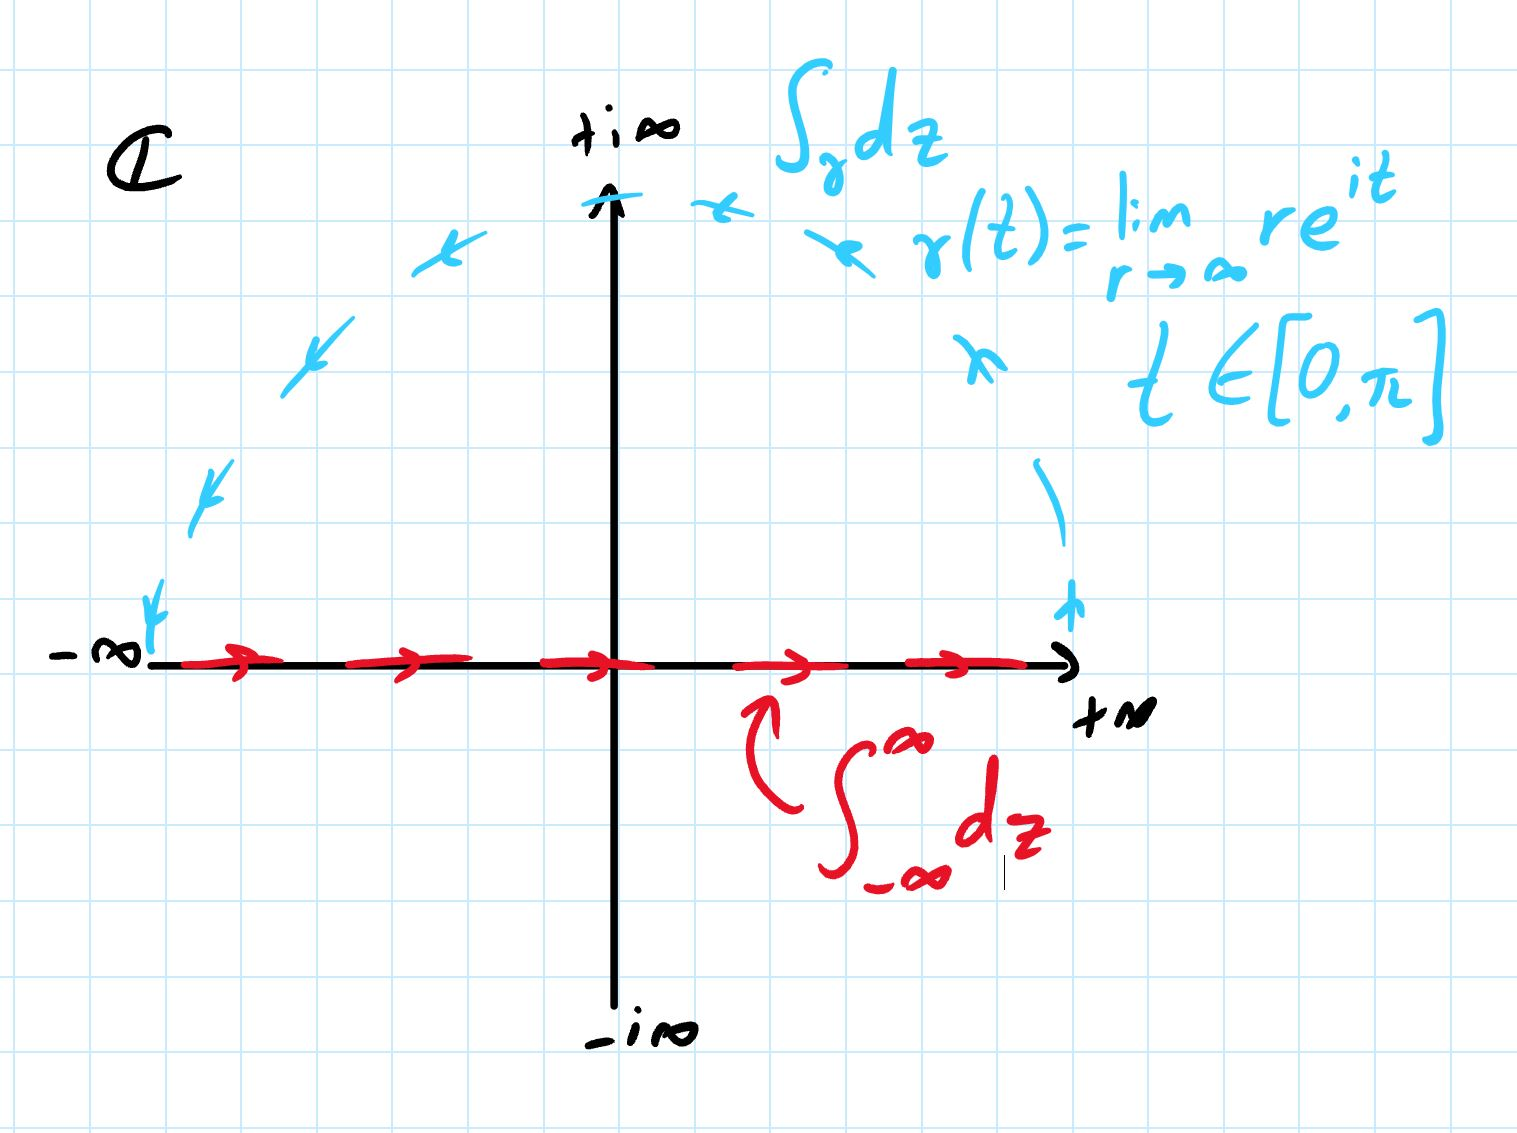
\includegraphics[width=0.8\linewidth]{2018/10/20180704_1.JPG}
\caption{An illustration of closing the contour for a real integral (in red) so we can use the Cauchy integral formula to perform the integral. The integral along the light blue curve $\int_\gamma dz$ contributes nothing to the overall integration, so we can use it to close the contour out at $+i\infty$. Note the curve runs counterclockwise. If it ran clockwise, we would pick up a minus sign.}
\end{figure}

How do we decide whether to close the contour in the upper or lower half-plane? Notice that in the upper half-plane, $z=x+iy$ for $y>0$, so $e^{iz}=e^{i(x+iy)}=e^{-y}e^{ix}$ with $y>0$. Therefore, $e^{iz}$ is exponentially damped in the upper half-plane and contributes basically zero to the overall integral. So we can close the curve ''for free'' and write
$$\Int dz \frac{e^{iz}}{z-z_0}=\oint dz \frac{e^{iz}}{z-z_0}=2\pi i e^{iz_0}$$
if $z_0$ has imaginary part $>0$ (is inside the contour) and $0$ otherwise. Thanks, Cauchy integral formula.

In fact, the formula lends itself to an even better generalization, the \term{Cauchy residue theorem}. It states that $$\oint_C f(z)dz = 2\pi i\cdot \text{sum of the residues of }f(z) \text{ inside } C,$$ where the integral around $C$ is in the counterclockwise direction, and a \term{residue} is basically the value at the function at the pole if it didn't have that pole. Quick example: for the function $f(z)=\frac{z}{(1+z)(3-z)}$, $f(z)$ has a pole at $z=3$. The residue $R(3)$ of $f(z)$ at $z=3$ is simply $R(5)=\frac{z}{1+z}|_{z=3}=\frac{3}{4}.$

So to summarize, close the contour based on what the integrand is doing at $\pm i\infty$. Check which poles are inside your contour, and plug up the singularities one at a time to compute the residues. Sum up the residues, multiply by $2\pi i$, and you've got the value of your integral.

Returning to the problem at hand, we wish to compute the integral
$$\int dk^0 \frac{e^{i k^0 x^0}}{(k^0)^2-(\omega_k^2-i\e)}.$$ We have two poles at $\pm\sqrt{\omega_k^2-i\e}$, which in the $\e\to 0$ limit become $+\omega_k-i\e$ and $-\omega_k+i\e$. Therefore, we rewrite as
$$\Int dk^0 \frac{e^{i k^0 x^0}}{(k_0-(\omega_k-i\e))(k_0-(-\omega_k+i\e))}.$$
Since $e^{ik^0x^0}$ is exponentially damped in the upper half-plane, we close the contour at $+i\infty$, enclosing the pole at $-\omega_k+i\e$ (recall $\omega_k$ is real and $\e$ is positive). Therefore, calculating the residue, this integral comes out to
$$2\pi i \frac{e^{-i\omega_k x^0}}{-2\omega_k}$$
(letting $\e\to 0$) and we conclude that for $x^0>0$,
$$\Delta_F(x)=-i \int \frac{d^3 k}{(2\pi)^3 2\omega_k}e^{-i(\omega_k t- \vec{k}\cdot \vec{x})}.$$
A similar calculation holds for $x^0 < 0$, so we recover the form of the Feynman propagator which correctly accounts for the sign of $x^0$.

\section{Saturday, October 20, 2018}
    Previously, we defined the exponential map
$$g(t)=\exp(tX)=\sum_{l=0}^\infty \frac{1}{l!}t^l X^l.$$ In the exercises (Example Sheet 1, Q10) we'll check explicitly that for $X\in L(SU(n)),$ we have $\exp(tX)\in SU(N) \forall t\in \RR.$ We'll also show in a separate question (Example Sheet 2, Q1) that for a choice of $X\in L(G)$ with $G$ a Lie group and $J$ an interval with $J\subset \RR$, $S_X=\set{g(t)=\exp(tX} \forall t \in J \subset \RR$ forms an abelian subgroup of $G$. We call this a one-parameter subgroup.

Now we might be interested to reconstruct $G$ from $L(G)$. Setting $t=1$ we get a map $$\exp:L(G)\to G,$$ and this map is one-to-one in some neighborhood of the identity $e$. (We haven't proved this but it's true.) Then given $X,Y\in L(G)$ we would also like to reconstruct the group multiplication from the Lie algebra, and the solution to this will be the \term{Baker-Campbell-Hausdorff (BCH) formula}.

For $X,Y\in L(G)$ define
$$g_X=\exp(X), g_Y=\exp(Y)$$
and
$$g_X^\epsilon(x)=\exp(\epsilon X), g_Y^\epsilon(Y)=\exp (\epsilon Y).$$
Then their product is
$$g_X g_Y= \exp(Z)\in G, z\in L(G).$$ Expanding out, we find that
$$\left(\sum_{l=0}^\infty \frac{X^l}{l!}\right)\left(\sum_{l'=0}^\infty \frac{Y^{l'}}{l' !}\right)=\sum_{m=0}^\infty \frac{Z^m}{m!}$$
and one may work out the terms order by order-- it looks something like this.
$$Z=X+Y+\frac{1}{2}[X,Y]+\frac{1}{12}([X,[X,Y]]-[Y,[X,Y])+\ldots \in L(G),$$
and we know that this is in the Lie algebra since it is made up of $X$, $Y$, and brackets of $X$ and $Y$ which are guaranteed to be in the Lie algebra. Moreover this generalizes to Lie algebras that aren't matrix groups, since the construction only uses the vector space structure of $L(G)$ and the Lie bracket.

$L(G)$ therefore determines $G$ in a neighborhood of the identity (up to the radius of convergence of $\exp Z$, anyway). The exponential map may \emph{not} be globally one-to-one, however. For instance, it is not surjective when $G$ is not connected.
\begin{exm}
For $G=O(n)$, 
$$L(O(n))=\set{X\in \text{Mat}_n(\RR): X+X^T=0}.$$ 
Then $X\in L(O(n)) \implies \text{Tr} X=0.$ Now let $g=\exp(X)$, $X\in L(O(n)$. We have a nice identity\footnote{To prove this, consider a basis where $X$ is diagonal, $X_{ij}=\delta_{ij}\lambda_i,$ with $\lambda_i$ the eigenvalues of $X$. Then powers of $X$ are given by $X_{ij}^n=\delta_{ij}\lambda_i^n$ and the matrix exponential is simply the matrix with the exponential of each diagonal entry, $(\exp X)_{ij}=\delta_{ij} \exp(\lambda_i).$ It follows that the determinant of the exponential is $\Pi_i \exp(\lambda_i)= \exp(\sum_i \lambda_i)$, which is just the exponential of the sum of the eigenvalues.} that
$$\det (\exp X) = \exp(\text{Tr} X),$$
and since $\text{Tr} X = 0, \det (\exp X) = 1$. Therefore $\exp(X)\in SO(n) \subset O(n).$

We'll mention another non-proven fact-- for $G$ compact, the image of the $\exp$ map is the connected component of the identity. This squares with what we just showed for $O(n).$
\end{exm}

Our map can also fail to be injective when $G$ has a $U(1)$ subgroup. 
\begin{exm}
For $G=U(1),$ we have 
$$L(U(1))=\set{X=ix \in \CC: x\in \RR}.$$
Thus $g=\exp(X)=\exp (ix),$
but the Lie algebra elements have a degeneracy where $ix$ and $ix+2\pi i$ yield the same group element (by Euler's formula) under the $\exp$ map.
\end{exm}

Let's now return to our discussion of $SU(2)$ vs. $SO(3).$ We saw that $L(SU(2))\simeq L(SO(3)),$ and so we can construct a double-covering, i.e. a globally 2:1 map
$d:SU(2)\to SO(3)$ with $d: A\in SU(2) \mapsto d(A) \in SO(3).$ One can write the map explicitly as
$$d(A)_{ij} =\frac{1}{2} \text{tr}_2 (\sigma_i A \sigma_j A^\dagger).$$
However, $d$ is not one-to-one since $d(A)=d(-A).$ But we'll explore the properties of this map more on Example Sheet 2. Recall that $SU(2)\simeq S^3$ the three-sphere. If we therefore quotient out by this map, this is the same as identifying antipodal points on the three-sphere. That is, this map provides an isomorphism
$$SO(3) \simeq SU(2)/\ZZ_2$$
where $\ZZ_2=\set{I_2,-I_2}$ is the centre of $SU(2)$, which is a discrete (normal) subgroup of $SU(2)$.\footnote{A subgroup $H\subset G$ is normal if $gHg^{-1}=H \forall g\in G$. Then we define the quotient $G/H$ to be the original group under identification of the equivalence classes corresponding to the elements of the normal subgroup. Normal subgroups ``tile'' the group-- they separate it into distinct cosets, so it makes good sense to quotient (``mod out'') by a normal subgroup.}

Put another way, $SO(3)$ is the upper hemisphere $U^+$ of the three-sphere $S^3$ with antipodal identification on the equation $S^2$. But the upper hemisphere $U^+$ is homeomorphic to the three-ball $B_3$, with $\p B_3 = S^2$. So the quotient is the same thing as chopping $S^3$ in half, flattening out the upper hemisphere $U^+\to B^3$ and identifying antipodal points on the equator $\p B_3 =S^2.$

\begin{defn}
For a Lie group $G$, a \term{representation} $D$ is a map
$$D:G\to \text{Mat}_n(F)\text{ with }\det M \neq 0.$$
Equivalently we could call this a map to $GL(n,F).$ That is, a representation takes us from a Lie group to a set of invertible matrices such that the group multiplication is preserved by the map,
$$\forall g_1,g_2\in G, D(g_1)D(g_2)=D(g_1g_2).$$
For a Lie group specifically, we also require that the manifold structure is preserved, so that $D$ is a smooth map (continuous and differentiable). When the map is injective, we say that the representation is \term{faithful}, but in general representations may be of lower dimension (e.g. the trivial representation where we send every group element to the identity matrix).
\end{defn}

\begin{defn}
For a Lie algebra $\fg,$ a \term{representation} $d$ is a map
$$d:\fg\to \text{Mat}_n(F).$$
Note that the zero matrix is part of the Lie algebra since a Lie algebra has a vector space structure, so it won't make sense to require that $\det M\neq 0$. All we require is that this map $d$ has the properties that
\begin{itemize}
    \item it preserves the bracket operation, $[d(X_1),d(X_2)]=d([X_1,X_2])$ where $[d(X_1),d(X_2)]$ is now the matrix commutator.
    \item the map is linear, so it preserves the vector space structure: $d(\alpha X_1+\beta X_2)=\alpha d(X_1)+\beta d(X_2) \forall X_1,X_2\in \fg, \a,\beta \in F$.
\end{itemize}
\end{defn}

The \term{dimension of a representation} is then the dimension $n$ of the corresponding matrices we're using in the image of our map $d$ or $D$. The matrices in the image naturally act on vectors living in a vector space $V=F^n$ (i.e. column vectors with $n$ entries in the field $F$). We call this the \term{representation space}.

Next time, we'll show that representations of the Lie group have a natural correspondence to representations of the Lie algebra.
    
\section{Tuesday, October 23, 2018}
    Today, we'll introduce Wick's formula and contractions, calculate some more scattering amplitudes, and maybe see our first Feymman diagrams for calculating amplitudes in a more convenient way.

First, we complete the calculation of the order $g$ scattering amplitude from last time. We were interested in meson decay, where we prepared initial and final states
$$\ket{i}=\sqrt{2E_p}a_{\vec p}^\dagger \ket{0}$$
and
$$\ket{f}=\sqrt{4E_{q_1}E_{q_2}}b_{\vec q_1}^\dagger c_{\vec q_2}^\dagger \ket{0},$$
and we were interested in the scattering amplitude $\bra{f}S \ket{i}$. To leading order, we found that
$$\bra{f}S\ket{i}=-ig \bra{f}\int d^4 x \psi^* (x) \psi(x) \phi(x) \ket{i} + O(g^2),$$
and we'll see how to compute this.

We know how to expand each of these fields in terms of creation and annihilation operators, and we want to make sure that the initial state and final state are indeed proportional to each other so that this QFT amplitude will be reduced to a c-function of the four-momenta (i.e. it is just a number). 

For instance, in $\phi$ we will have both $a_{\vec p}^\dagger$ and $a_{\vec p}$ terms, but our initial state already has an $a^\dagger$. So the $a^\dagger$ bit of $\phi$ acting on $\ket{i}$ will produce a two-meson state which the $\psi$s won't touch, which means that its inner product with $\bra{0}$ will be zero. (Alternately you can think of the $a^\dagger$ from $\phi$ as acting on the $\bra{0}$ on the left, commuting through the $\psi$s. That is, $a_{\vec k}\ket{0}=0\implies \bra{0} a_{\vec k}^\dagger =0.$) So our matrix element takes the form
$$\bra{f}S\ket{i}=-ig \bra{f} \int d^4x \psi^*(x) \psi(x)\int \frac{d^3k}{(2\pi)^3}\frac{\sqrt{2E_p}}{\sqrt{2E_k}}(a_k a_p^\dagger e^{-ik\cdot x}+a_k^\dagger a_p^\dagger e^{ik\cdot x})\ket{0},$$
but this second term is just zero and we can switch the $a_k, a_p^\dagger$ at the cost of a delta function $(2\pi)^3 \delta^3(\vec k -\vec p)$, which allows us to do the integral over $d^3k$.

We get
\begin{eqnarray*}
\bra{f}S\ket{i}&=&-ig\bra{f} \int d^4x \psi^* \psi(x)e^{-ip\cdot x}\ket{0}\\
&=&-ig \bra{0} \int \frac{d^4x}{(2\pi)^6}\frac{d^3k_1 d^3k_2}{\sqrt{4E_{k_1}E_{k_2}}} \sqrt{4E_{q_1}E_{q_2}} c_{q_2}b_{q_1} (b_{k_1}^\dagger e^{ik_1\cdot x}+c_{k_1} e^{-ik_1 \cdot x})(b_{k_1} e^{-ik_2\cdot x}+c_{k_2}^\dagger e^{ik_2 \cdot x})e^{-ip\cdot x} \ket{0}.
\end{eqnarray*}
Only the $b^\dagger$ and $c^\dagger$ terms survive, and taking the appropriate commutators gives us delta functions over the momenta. That is,
\begin{eqnarray*}
\bra{f}S\ket{i}&=&-ig\bra{0}\int d^4x e^{i(q_1+q_2-q)\cdot x}\ket{0}\\
&=&-ig\delta^4(q_1+q_2-p)(2\pi)^4
\end{eqnarray*}
where this delta function simply imposes overall 4-momentum conservation. Note that this is a matrix element, not a probability yet. To actually turn this into a measurable probability, we must take the mod squared and integrate over the possible outgoing momenta $q_1,q_2$-- we'll defer this to later.


We'll now discuss \term{Wick's theorem} for a real scalar field. We wish to compute quantities like
$$\bra{f}T\set{H_I(x_1)\ldots H_I(x_n)}\ket{i},$$
the amplitude of some time-ordered product-- remember that Dyson says we ought to be evolving our states with time-ordered products. Our life would be easier if we worked in terms of normal-ordered products instead, where the $a$s are on the RHS and the $a^\dagger$s are on the LHS. This would let us easily see which terms contribute to the final amplitude (e.g. which $a$s cancel particles created by $a^\dagger$s on the RHS).

Let's compute a simple example first: write
$$\phi(x)\equiv \phi^+(x)+\phi^-(x)$$
where
$$\phi^+ (x)\equiv \int \frac{d^3p}{(2\pi)^3}\frac{1}{\sqrt{2E_p}} a_p e^{-ip\cdot x}$$
and
$$\phi^-(x)\equiv \int \frac{d^3p}{(2\pi)^3}\frac{1}{\sqrt{2E_p}} a_p^\dagger e^{+ip\cdot x}.$$
If we look at the case $x^0>y^0$, the time-ordered product $T\{\phi(x)\phi(y)\}$ takes the form
\begin{eqnarray*}
T\set{\phi(x)\phi(y)}&=&\phi(x)\phi(y)\\
&=&(\phi^+(x)+\phi^-(x))(\phi^+(y)+\phi^-(y))\\
&=&\phi^+(x)\phi^+(y)+\phi^-(x)\phi^-(y)+\phi^-(y)\phi^+(x)+\phi^-(x)\phi^+(y)+[\phi^+(x),\phi^-(y)]\\
&=&:\phi(x)\phi(y):+D(x-y)
\end{eqnarray*}
where we've collected terms with all the $\phi^+$ terms to the right of the $\phi^-$ terms into the normal-ordered product $:\phi(x)\phi(y):$. If we had $y^0>x^0$ instead, we would get
$$T\set{\phi(x)\phi(y)}=:\phi(x)\phi(y):+D(y-x).$$
Putting these together, we see that
$$T\set{\phi(x)\phi(y)}=:\phi(x)\phi(y):+\Delta_F(x-y),$$
where $\Delta_F$ is simply the Feynman propagator. It's important to note that while the time-ordered and normal-ordered products are both operators, their difference is $\Delta_F$, a c-function.

\begin{defn}
We define a \term{contraction} of a pair of fields in a string in a string (denoted by a square bracket between the two fields) to mean replacing the two contracted fields by their Feynman propagator.

For instance, we saw that
$$T\set{\phi(x)\phi(y)}=:\phi(x)\phi(y)+\overbrace{\phi(x)\phi(y)}.$$
\end{defn}

Wick's theorem states that
$$T\set{\phi(x_1)\ldots \phi(x_n)}=:\phi(x_1)\ldots \phi(x_n):+:\text{all possible contractions}:.$$
Since all normal ordered terms kill the vacuum state, this allows us to immediately compute amplitudes like
$$\bra{0}T\set{\phi_1\ldots \phi_4}\ket{0}=\Delta_F (x_1-x_2)\Delta_F(x_3-x_4)+\Delta_F(x_1-x_3)\Delta_F(x_2-x_4)+\Delta_F(x_1-x_4)\Delta_F(x_2-x_3).$$

The proof of Wick's theorem is by induction. Suppose it holds for $T\set{\phi_2\ldots \phi_n}$. Then (see textbooks for detail)
$$T\set{\phi_1 \phi_2\ldots \phi_n}=(\phi_1^+ +\phi_1^-)[:\phi_2\ldots \phi_n+:\text{all contractions of }\phi_2\ldots \phi_n:].$$
The $\phi_1^-$ is okay where it is, while the $\phi_1^+$ must be commuted to the RHS of the $\phi_2\ldots \phi_n$ terms. Each commutator past the $x_k$ term in $\phi_2\ldots \phi_n$ gives us a $D(x_1-x_k)$, which is equivalent to a contraction between $\phi_1$ and $\phi_k$.

Wick's theorem has some immediate consequences. For instance,
$$\bra{0}T \phi_1\ldots \phi_n\ket{0}=0$$ if $n$ is odd (since one $\phi$ is always left out of the contractions) and it is
$$\sum_{i_1,\ldots,i_n}\Delta_F (x_{i_1}-x_{i_2})\Delta_F(x_{i_3}-x_{i_4})\ldots \Delta_F(x_{i_{n-1}}-x_{i_n})$$
where the sum is taken over symmetric permutations of $i_1,\ldots,i_n$.

Note that Wick's theorem also has a generalization to complex fields $\psi\in \CC$, e.g.
$$T(\psi(x)\psi^*(y))=:\psi(x)\psi^*(y):+\Delta_F(x-y)$$
where the contraction of $\psi(x)\psi^*(y)\equiv \Delta_F(x-y)$ and the contractions of two $\psi$s or two $\psi^*$s is zero.

\section{Thursday, October 25, 2018}
    Today, we'll consider the consequences of some specific representations and their structures.

\begin{defn}
Two representations $R_1$ and $R_2$ are \term{isomorphic} if $\exists$ a matrix $S$ such that
$$R_2(X)=S R_1(X)S^{-1} \, \forall X\in \fg.$$
Note this must be the same matrix $S$: that is, $R_2$ and $R_1$ are related by a change of basis. If so, we denote this as $$R_1\cong R_2.$$
\end{defn}
\begin{defn}
A representation $R$ with representation space $V$ has an \term{invariant subspace} $U\subset V$ if
$$R(X)u\in U \, \forall X\in \fg, u\in U.$$
(This is equivalent to our ideals in Lie algebras and normal subgroups in group theory.)

Any representation has two trivial invariant subspaces: they are the vector $U=\set{0}$ and $U=V$ the whole representation space.
\end{defn}
\begin{defn}
An \term{irreducible representation} (irrep) of a Lie algebra has no non-trivial invariant subspaces.
\end{defn}

With these definitions in hand, let's look at the representation theory of $L(SU(2))$. It's useful to us to write down a basis for the Lie algebra $L(SU(2))$:
$$\set{T^a=-\frac{1}{2}i\sigma_a,a=1,2,3}$$
with $\sigma_a$ the Pauli matrices. We calculated the structure constants:
$$[T^a,T^b]=f^{ab}_c T^c$$ with $f^{ab}_c=\epsilon_{abc}$ (the alternating tensor/symbol) and $a,b,c=1,2,3$. Let's do something kind of strange-- we'll write a new complex basis,
\begin{align*}
    H&\equiv \sigma_3 = 
        \begin{pmatrix}
            1&0\\0&-1
        \end{pmatrix}\\
    E_+ &\equiv \frac{1}{2}(\sigma_1+i\sigma_2) = 
        \begin{pmatrix}
            0&1\\0&0
        \end{pmatrix}\\
    E_-&\equiv\frac{1}{2}(\sigma_1 - i\sigma_2)= 
        \begin{pmatrix}
            0&0\\1&0
        \end{pmatrix}.
\end{align*}
This is really a basis for a somewhat bigger space, the complexified Lie algebra
$$L_\CC (SU(2))=\text{Span}_\CC\set{T^a, a=1,2,3}.$$

For now, we'll simply note that for $X\in L(SU(2))$, we can certainly rewrite $X$ as
$$X=X_H H + X_+ E^++ X_- E^-,$$
where $X_H\in i\RR$ and $X_+=-(\bar X_-)$ (where bar indicates complex conjugation, as usual). This is called the Cartan-Weyl basis for $L(SU(2))$.\footnote{We've been writing $L(G)$ to distinguish the Lie algebra from the corresponding Lie group $G$, but other texts may use the convention of writing $su(2)$ using lowercase letters or the Fraktur script $\mathfrak{su}(2)$ for the Lie algebra. Just a convention to be aware of.}
In this basis, a general element takes the form
%
$$X=\begin{pmatrix}
    X_H & X_+\\
    X_-&-X_H
\end{pmatrix}.$$
%
This is certainly traceless, and $X\in L(SU(2))\iff$ $X$ is antihermitian, i.e. $X_H\in i\RR, X_+ = -(\bar X_-)$.

This basis has some nice properties. For instance, we see that
\begin{align*}
    [H,E_\pm] &= \pm 2 E_\pm\\
    \text{ and } [E_+,E_-] &= H.
\end{align*}
Hence the ad map takes a very simple form:
$\ad_H(E_\pm)=\pm 2 E_\pm, \ad_H(H)=0.$
We also have $ad_H(X)=[H,X]\forall X \in L_\CC(SU(2))$. This describes a general $X$, but note that in this basis, our basis vectors $\set{E_+,E_-,H}$ are eigenvectors of
$$\ad_H:L(SU(2))\to L(SU(2)).$$
That is, we have chosen a basis that diagonalizes the ad map, and its eigenvalues $\set{+2,-2,0}$ are called \term{roots}.

\begin{defn}
Consider a representation $R$ of $L(SU(2))$ with a representation space $V$. We \emph{assume} that $R(H)$ is also diagonalizable. Then the representation space $V$ is spanned by eigenvectors of $R(H)$, with
$$R(H)v_\lambda = \lambda v_\lambda: \lambda \in \CC.$$
The eigenvalues $\lambda$ are called \term{weights} of the representation $R$.
\end{defn}
\begin{defn}
For such a representation, we call $E_\pm$ the \term{step operators} (cf. the ladder operators from quantum mechanics).
\end{defn}
The step operators are so named because their representations take eigenvectors of $R(H)$ with eigenvalue $\lambda$ to new eigenvectors of $R(H)$ with new eigenvalues $\lambda \pm 2$. That is, if $R(H)v_\lambda = \lambda v_\lambda$, then
\begin{align*}
    R(H)R(E_\pm)v_\lambda &= (R(E_\pm)R(H) + [R(H),R(E_\pm)]) v_\lambda\\
    &=(\lambda \pm 2) R(E_\pm)v_\lambda.
\end{align*}
%We see that the vectors $R(E_\pm)v_\lambda$ we got from acting on eigenvectors of $R(H)$ with the step operators are also 

Note that a finite dimensional representation $R$ of $L(SU(2))$ must have a highest weight $\Lambda \in \CC$, or else we could just keep acting with the raising operator $E_+$ to get more linearly independent vectors. (We can play a similar trick assuming only a lowest weight-- this is what led us to the ladder of harmonic oscillator states.)
If there is a highest weight, then we have
\begin{align*}
    R(H)v_\Lambda &= \Lambda v_\Lambda\\
    R(E_+)v_\Lambda &= 0.
\end{align*}
If $R$ is irreducible, then all the remaining basis vectors of $V$ can be generated by acting on the highest-weight eigenvector $v_\Lambda$ with $R(E_-)$ (that is, there is only one ladder of states to construct). By doing this $n$ times, we get some new lowered states
$$V_{\Lambda-2n}=(R(E_-))^n v_\Lambda, n\in \NN.$$
What happens if we now try to raise the lowered states back up? The result is as nice as we could have hoped-- we will get back our old states, up to some normalization.
\begin{align*}
    R(E_+)v_{\Lambda-2n} &= R(E_+) R(E_-)v_{\Lambda-2n+2}\\
    &= (R(E_-)R(E_+)+[R(E_+),R(E_-)]) v_{\Lambda -2n + 2}\\
    &= (R(E_-)R(E_+)+R(H)) v_{\Lambda -2n + 2}\\
    &= R(E_-)R(E_+)v_{\Lambda -2n+2} + (\Lambda -2n+2) v_{\Lambda-2n+2}.
\end{align*}
where we have used the fact that the representation preserves the bracket structure.

Looking at the lowest-$n$ cases, we can now take $n=1$ to find
$$R(E_+)v_{\Lambda-2}=\Lambda v_\Lambda$$
and then for $n=2$,
\begin{eqnarray*}
R(E_+)v_{\Lambda-4}&=&R(E_-)R(E_+)v_{\Lambda-2}+(\Lambda-2)v_{\Lambda-2}\\
&=&\Lambda R(E_-)v_\Lambda +(\Lambda-2)v_{\Lambda-2}\\
&=&(2\Lambda-2) V_{\Lambda-2}.
\end{eqnarray*}
Proceeding by induction, we find that we can always use the relations for lower $n$ to eliminate the $R(E_+)$s at any $n$ we like and write the final result in terms of the next state up. That is,
$$R(E_+)v_{\Lambda -2n}= r_n v_{\Lambda-2n+2}.$$
Plugging this into our general equation for $R(E_+)v_{\Lambda-2n},$ we get a recurrence relation\footnote{Clearly, the left side of our original recurrence relation just becomes $r_n v_{\Lambda-2n+2}$. On the right side, we've left out a few steps. $R(E_-)R(E_+)v_{\Lambda-2n+2}=R(E_-)R(E_+)v_{\Lambda-2(n-1)}=R(E_-)r_{n-1}v_{\Lambda -2n+4} = r_{n-1}v_{\Lambda-2n+2}.$ Pull out the $v_{\Lambda-2n+2}$s everywhere and you're left with the recurrence relation.}:
$$r_n = r_{n-1}+\Lambda -2n+2$$
with the single boundary condtion that $R(E_+)v_\Lambda =0$. This implies that $r_0=0,$ so we use this to find that our recurrence relation takes the form
$$r_n=(\Lambda+1-n)n.$$

In addition, a finite-dimensional representation must also have a lowest weight $\Lambda-2N$ (recall $N$ is the dimension of the representation). That is, we have some lowest weight vector $v_{\Lambda-2N}\neq 0$ such that
%
$$R(E_-)v_{\Lambda-2N}=0\implies v_{\Lambda-2N-2}=0 \implies r_{N+1}=0.$$
%
But using the recurrence relation, $r_{N+1}$ vanishing means that 
%
$$(\Lambda - N)(N+1)=0 \implies \Lambda= N \in \ZZ_{\geq 0}.$$
%
This completes the characterization of the representation theory of $L(SU(2))$. We conclude that a finite dimensional irrep $R_\Lambda$ of $L(SU(2))$ can be described totally by a highest weight $\Lambda \in \ZZ_{\geq 0}$ and it comes with a remaining set of weights
$$S_{R_\Lambda}=\set{-\Lambda, -\Lambda+2,\ldots \Lambda-2,\Lambda}\subset \ZZ,$$
where $$\dim(R_\Lambda)=\Lambda+1.$$

\begin{exm}
Let's take some explicit cases. $R_0$ has dimension $1$ ($d_0$, the trivial representation), $R_1$ has dimension $2$ ($d_f$, the fundamental representation), and $R_2$ has dimension 3 ($d_{Adj}$, the adjoint representation).
\end{exm}

This is precisely equivalent to the theory of angular momentum in quantum mechanics but with a different normalization-- in QM, our spin states had single integer steps but with $j_{max}=n/2, n\in\NN.$ This happens because the angular momentum operators obey the same bracket structure (i.e. fail to commute) in exactly the same way as the basis elements of the Lie algebra $L(SU(2))$. 
    
\section{Saturday, October 27, 2018}
    Some remarks from last time. In terms of the original basis vectors, our basis for $SU(2)$ was
$$H=2i T^3, E_\pm i(T^1 \pm i T^2$$
with $T^a=-\frac{1}{2}i \sigma_a, a=1,2,3.$ Conversely $T^3=H/2i, T^1=\frac{1}{2i}(E_+ + E_-), T^2= -\frac{1}{2}(E_+-E_-).$

It follows that a representation $R$ of $L_\CC(SU(2))$, $R(H2),R(E_+),R(E_-)$ gives a representation of $L(SU(2))$ by applying our representation to the original basis elements, e.g.
$$R(T^1)=\frac{1}{2i} R(E_++ E_-)=\frac{1}{2i}(R(E_+)+R(E_-).$$

Today we'll consider the $SU(2)$ representation from $L(SU(2))$ representations. That is, we'll look at the connection between the representation of a Lie algebra $L(G)$ and the representation of the original Lie group $G$.

The punchline from last time was that finite-dimensional irreps of $L(SU(2))$ can be labeled by the highest weight $\Lambda_\in \ZZ_{\geq 0},$ with a weight set
$$S_\Lambda=\set{-\Lambda, \Lambda+2,\ldots, \Lambda-2, +\Lambda}\subset \ZZ.$$
We had $\dim(R_\Lambda)=\Lambda+1$.

To a physicist, this is simply a complicated way of expressing angular momentum in quantum mechanics. Recall that the total angular momentum is orbital $+$ spin angular momentum. We had our $\vec J$ operator,
$$\vec J=(J-1,J_2,J_3)$$ with eigenstates (e.g. of $J_3$) labeled by $j\in \ZZ/2, j\geq 0.$ We then had
$$m\in \set{-j,j+1,\ldots,+j}$$
such that
$$\hat J_3\ket{j,m}=m\ket{j,m}$$
and the total angular momentum $J^2$ with
$$\hat J^2 \ket{j,m}=j(j+1)\ket{j,m}.$$

We can set up the correspondence
$$J_3=\frac{1}{2}R(H)$$
and
$$J_\pm = J_1\pm i J_2 = R(E_\pm)$$
so that the highest weight $\Lambda$ of the representation corresponds to 
$$\Lambda = 2j \in \ZZ$$ and a general weight $\lambda \in S(R)$ corresponds to the angular momentum along a particular axis,
$$\lambda = 2m\in \ZZ.$$
The eigenvector $v_\Lambda$ thus corresponds to
$v_\Lambda \sim \ket{j,j}$ and similarly $v_\lambda \sim \ket{j,m}.$
This explains in an algebraic context why $m$ ranges from $-j$ to $j$ in integer steps, with $j$ a positive half-integer. Fixing $\Lambda$ is equivalent to choosing the total angular momentum, and fixing $\lambda$ is then choosing the angular momentum along a particular axis (e.g. $J_3$).

Recall that locally we can parametrize group elements $A\in SU(2)$ using the exponential map,
$$A=\exp(X), X\in L(SU(2)).$$
Starting from the irreducible representations $R_\Lambda$ of $L(SU(2))$ defined above, we can then define the representation
$$D_\Lambda(A)\equiv \exp (R_\Lambda(X)), \Lambda \in \ZZ_{\geq 0}.$$
Recall that $SU(2)$ and $SO(3)$ have the same Lie algebra. In general this will yield a valid representation of $SU(2)$ but \emph{not} of $SO(3)\simeq SU(2)/\ZZ_2.$ For this to be a representation of $SO(3)$, we must further require that it is well-defined on the quotient by the center of the group $\set{I_2,-I_2},$ i.e.
$$D_\Lambda(-I_2)=D_\Lambda(I_2) \iff D_\Lambda(-A)=D_\Lambda(A) \forall A\in SU(2).$$

Let's check explicitly if that holds. First note that we can write
$$-I_2 = \exp (i \pi H)$$
(from the explicit form of $H$-- check this). Now we'll pass to the representation $D_\Lambda$:
$$D_\Lambda(-I_2)=D_\Lambda(\exp(i\pi H)) = \exp(i\pi R_\Lambda(H)).$$
But $R_\Lambda(H)$ has eigenvalues $\lambda\in\set{-\Lambda,\Lambda+2,\ldots,+\Lambda}$, so the matrix on the left $D_\Lambda(-I_2)$ must have the same eigenvalues (after exponentiation) $$\exp(i\pi \lambda)= \exp(i\pi \Lambda)=(-1)^\Lambda$$ since $\lambda$ goes in steps of $2$.
Therefore we find that
$$D_\Lambda(-I_2)=D_\Lambda(I_2)=(I)_{(\Lambda+1)\times (\Lambda+1)}\iff \Lambda \in 2\ZZ.$$
That is, $\Lambda$ must be even. In this case,
$\Lambda \in 2 \ZZ \implies D_\Lambda$ is a representation of $SU(2)$ and $SO(3)$, whereas $\Lambda \in 2 \ZZ+1 \implies D_\Lambda$ is a representation of $SU(2)$ but \emph{not} of $SO(3)$. Sometimes we call this a ``spinor representation'' (i.e. half-integer spin) of $SO(3)$, but these aren't really representations of $SO(3)$-- really, they're representations of the double cover $SU(2)$.

This reveals something a bit interesting-- the true rotation group of the physical world we live in is not $SO(3)$ but $SU(2)$. The particles which see these complex rotations are exactly the particles with half-integer spin.

\subsection*{New representations from old} 
\begin{defn}
If $R$ is a representation of a real Lie algebra $\fg$, we define a \term{conjugate representation} by
$$\bar R(X)=R(X)^* \forall X\in \fg.$$
It's an exercise to check that this really is a representation-- see example sheet 2. Note that sometimes $\bar R \simeq R$, so the new representation is isomorphic to the old one.
\end{defn}
\begin{defn}
Given representations $R_1,R_2$ of a Lie algebra with corresponding representation spaces $V_1,V_2$ and dimensions $d_1,d_2$, we may define the \term{direct sum} of the representations, denoted
$$R_1 \oplus R_2.$$
The direct sum acts on the direct sum of the vector spaces, $$V_1 \oplus V_2 = \set{v_1 \oplus v_2: v_1 \in V_1,
v_2 \in V_2}.$$ The dimension of the new representation space is simply $\dim(V_1 \oplus V_2)=d_1 +d_2.$ The direct sum is then defined very simply by
$$(R_1 \oplus R_2)(X)\cdot (v_1 \oplus v_2)=(R_1(X)v_1)\oplus (R_2(X)v_2) \in V_1,V_2.$$
There's probably a nice commuting diagram for this in category theory. To make this more concrete, one can write $(R_1\oplus R_2)(X)$ as a block diagonal matrix with $R_1(X)$ in the upper left, $R_2(X)$ in the lower right. This is known as a \term{reducible} representation, i.e a representation which can be written as the direct sum of two (or more) representations.
\end{defn}

\begin{defn}
Given vector spaces $V_1,V_2$ with dimensions $d_1,d_2$, we define the \term{tensor product space} $V_1 \otimes V_2$. It's got a different structure than the more familiar Cartesian product-- our tensor product space is spanned by basis elements
$$v_1 \otimes v_2, v_1\in V_1,v_2\in V_2.$$
In particular, the tensor product space has dimension $\dim(V_1\otimes V_2)=d_1 \times d_2$.
However, the addition structure on the tensor product space is special. In a Cartesian product, it makes sense to add terms like $(0,1)+(1,0)=(1,1)$ (i.e. term-wise addition). But a tensor product is a formal product. In a tensor product, $\ket{0}\otimes \ket{1} + \ket{1}\otimes \ket{0}$ cannot be simplified any further. It only makes sense to add terms which share one of the terms, e.g. something like $(0,1)+(1,1)=(1,1).$ Tensor products are of particular interest in physics because when we consider the Hilbert space of a multi-particle state, it can be represented not as a direct product but a tensor product of the individual single-particle states.\footnote{For a simple example, consider two particle spin states taking discrete values. $\ket{a},\ket{b}\in \set{\ket{0},\ket{1}}$. Then the two-particle states are described by the tensor product space $\ket{a}\otimes\ket{b}$ (sometimes $\ket{a}\ket{b}$ or simply $\ket{ab}$), which is spanned by $\ket{00},\ket{01},\ket{10},\ket{11}$. It's obvious in this notation that it doesn't make sense to add states like $\ket{10}+\ket{01}$-- addition is only well-defined when at least one of the original basis states matches, e.g. $\ket{10}+\ket{11}=\ket{1}(\ket{0}+\ket{1})$.}

Given two linear maps $M_1:V_1\to V_1,M_2: V_2\to V_2,$ we can define the \term{tensor product map} $(M_1\otimes M_2): V_1\otimes V_2 \to V_1 \otimes V_2$ such that
$$(M_1\otimes M_2)(v_1\otimes v_2)=(M_1 v_1)\otimes (M_2 v_2) \in V_1\otimes V_2,$$
which may be extended naturally to all elements of $V_1\otimes V_2$ by linearity (since we have defined it on all basis vectors).
\end{defn}
\begin{defn}
Suppose we have two representations $R_1,R_2$ of a Lie algebra $\fg$ acting on representation spaces $V_1,V_2$. By definition, for $X\in\fg$ we have
$$R_1(X):V_1\to V_1, R_2(X):V_2\to V_2.$$
Then we can define a new representation, the \term{tensor product representation} $(R_1\otimes R_2)$ such that for each $X\in \fg$, we get
$$(R_1\otimes R_2)(X):V_1 \otimes V_2 \to V_1 \otimes V_2,$$
given explicitly by
$$(R_1\otimes R_2)(X)\equiv R_1(X) \otimes I_{V_2} + I_{V_1} \otimes R_2(X).$$
Here, I've denoted $I_{V_1}$ as the identity on $V_1$ and the same is true for $I_{V_2}$. We'll talk more about what this looks like and why it's defined this way next time.
\end{defn}
    
\section{Tuesday, October 30, 2018}
    Last time, we defined the tensor product of two representations. Suppose we have a Lie algebra $\fg$ and two representations $R_1,R_2$ with representation spaces $V_1,V_2$ respectively and dimensions $\dim(R_1)=d_1,\dim(R_2)=d_2$. Then the tensor product of these two representations acts on the representation space $V_1\otimes V_2$ and is defined such that $\forall X\in \fg,$
$$(R_1\otimes R_2)(X)=R_1(X)\otimes I_2 + I_1 \otimes R_2(X).$$
Here, $I_1,I_2$ are the identity maps on $V_1$ and $V_2$.  Note also that
$$(R_1\otimes R_2)(X) \neq R_1(X) \otimes R_2(X),$$
since this would be quadratic rather than linear in $X$ and would therefore fail to be a representation.

To make this more concrete, let us choose bases
\begin{eqnarray*}
B_1&=&\set{v_1^j; j=1,\ldots, d_1}\\
B_2 &=&\set{v_2^\alpha; \alpha = 1,\ldots, d_2}.
\end{eqnarray*}
Thus a basis for $V_1 \otimes V_2$ is
$$B_{1\otimes 2}=\set{v_1^j \otimes v_2^\alpha; j=1,\ldots, d_1, \alpha = 1,\ldots, d_2}.$$
The dimension of the new representation is therefore $\dim(R_1 \otimes R_2) = d_1d_2$ (i.e. it is spanned by $d_1d_2$ tensor products of the $d_1$ basis vectors of $V_1$ and the $d_2$ basis vectors of $V_2$).

The tensor product representation $R_1\otimes R_2$ is then given in a basis by
$$(R_1\otimes R_2)(X)_{a\alpha, j \beta}=R_1(X)_{ij} \underbrace{I_{\alpha \beta}}_{d_2\times d_2} + \underbrace{I_{ij}}_{d_1\times d_1} R_2(X)_{\alpha \beta}$$
where the identity matrices have the dimensions indicated.

\begin{defn}
We say that a representation $R$ with representation space $V$ has an \term{invariant subspace} $U\subset V$ if
$$R(X) u \in U \forall X\in \fg, u\in U.$$
Every representation space has two trivially invariant subspaces, $U=\set{0}$ and $U=\set{V}$. We then say that if $V$ has no non-trivial invariant subspaces, we call the corresponding representation an \term{irreducible representation} or \term{irrep} of $\fg$.
\end{defn}

If $R$ has an invariant subspace $U$, we may find a basis such that for all $X\in \fg$, the representation matrices take the block matrix form
$$
R(X)=
\left(
\begin{array}{c|c}
A(X) & B(X) \\
\hline
0 & C(X)
\end{array}
\right)
$$
where the elements of $U$ now take the form
$$\left(\begin{array}{c}
U\\ \hline
0
\end{array}\right).$$

\begin{defn}
Moreover, a \term{fully reducible representation} can be written as a direct sum of irreps, i.e. in some basis, $R$ takes a block diagonal form 
$$
R(X)=
\left(
\begin{array}{c|c|c|c}
R_1(X) &  & & \\
\hline
 & R_2(X) & & \\
\hline
& & \ddots & \\
\hline
& & & R_n(X)
\end{array}
\right)
$$
\end{defn}

It's an important fact that if $R_i, i=1,\ldots, m$ are finite-dimensional irreps of a simple Lie algebra then
$$R_1\otimes R_2 \otimes \ldots \otimes R_m$$ is fully reducible as some direct sum
$$R_1\otimes R_2 \otimes \ldots \otimes R_m\cong \tilde R_1 \oplus \tilde R_2 \oplus \ldots \oplus \tilde R_{\tilde m}.$$

Practically speaking, let's consider tensor products of $L(SU(2))$ representations. Let $R_\Lambda,R_{\Lambda'}$ be two irreps of $L(SU(2))$ with highest weights $\Lambda,\Lambda'$ and representation spaces $V_\Lambda,V_{\Lambda'}$, where $\Lambda,\Lambda' \in \ZZ_{\geq 0}$. We defined these last time-- these are just the spin states of particles with total spin $\Lambda/2,\Lambda'/2$. They have dimension
$$\dim(R_\Lambda)=\Lambda+1,\dim(R_{\Lambda'})=\Lambda'+1.$$
We can then form the tensor product representation $R_\Lambda \otimes R_{\Lambda'}$ with representation space spanned by the tensor products of basis vectors:
$$V_{\Lambda}\otimes V_{\Lambda'}=\text{span}_\RR \set{v\otimes v'; v\in V_\Lambda, v'\in V_{\Lambda'}}.$$
Now $\forall X\in L(SU(2))$ we have
$$(R_\Lambda \otimes R_{\Lambda'})(X)\cdot (V\otimes v') = (R_\Lambda(X) v)\otimes v'+ v \otimes (R_{\Lambda'}(X)v').$$
Since $L(SU(2))$ is simple, this gives a fully reducible representation of $L(SU(2))$ of dimension
$$\dim(R_\Lambda \otimes R_{\Lambda'}) = (\Lambda+1)(\Lambda'+1)$$
Then we can rewrite the tensor product as a direct product:
$$R_\Lambda \otimes R_{\Lambda'}=\bigoplus_{\Lambda'' \in \ZZ_{\geq 0}} L^{\Lambda''}_{\Lambda,\Lambda'}R_{\Lambda''}$$ for some non-negative integers $L^{\Lambda''}_{\Lambda,\Lambda'}$, which we call ``Littlewood-Richardson coefficients.'' That is, the various irreps appear in the direct sum with some multiplicity given by these coefficients.

Now recall that $V_\Lambda$ has a basis $\set{v_\lambda}$ where $\lambda$ specifies the weights,
$$\lambda \in S_\Lambda = \set{-\Lambda,-\Lambda+2,\ldots,+\Lambda}$$
where these $v_\lambda$ are eigenvectors of $R_\Lambda(H)$ such that
$$R_\Lambda(H)v_\lambda = \lambda v_\lambda.$$
Similarly $V_{\Lambda'}$ is equipped with a basis
$\set{v'_{\lambda'}}$ where 
$$\lambda' \in S_{\Lambda'} = \set{-\Lambda',-\Lambda'+2,\ldots,+\Lambda'}$$
and
$$R_{\Lambda'}(H)v'_{\lambda'}=\lambda' v'_{\lambda'}.$$
Therefore a basis for the representation space $V_\Lambda \otimes V_{\Lambda'}$ is given by
$$B_{\Lambda \otimes \Lambda'} = \set{v_\lambda \otimes v'_{\lambda'}; \lambda \in S_\lambda, \lambda' \in S_{\Lambda'}}.$$

Acting on a particular basis vector, we find that
\begin{eqnarray*}
(R_\Lambda \otimes R_{\Lambda'})(H)(v_\lambda \otimes v'_{\lambda'}&=&(R_\Lambda(H)v_\lambda) \otimes v'_{\lambda'}+v_\lambda \otimes (R_{\Lambda'}(H)v'_{\lambda'})\\
&=& (\lambda + \lambda')(v_\lambda \otimes v'_{\lambda'}).
\end{eqnarray*}
What we find is that the possible weights are therefore just sums of the individual $\lambda,\lambda'$. That is, the weight set of $R_\Lambda \otimes R_{\Lambda'}$ is simply
$$S_{\Lambda,\Lambda'}=\set{\lambda+\lambda': \lambda\in S_{\Lambda},\lambda'\in S_{\Lambda'}}.$$
Note that elements of this set can have degeneracy-- the same number can appear more than once!\footnote{Consider $\lambda=2,\lambda'=0$ and $\lambda=0,\lambda'=2$. Both of these will appear as terms in the set so the weight $2$ can appear twice. We'll see this concretely in a minute.} However, it's also true that if we look for the highest weight of the new tensor product representation, it is exactly $\Lambda+\Lambda'$, appearing with multiplicity one:
$$L^{\Lambda+\Lambda'}_{\Lambda,\Lambda'}=1.$$

Thus we may write
$$R_\Lambda \otimes R_{\Lambda'}=R_{\Lambda+\Lambda'}\oplus \tilde R_{\Lambda,\Lambda'}$$
where we have written the tensor product in terms of a new irrep $R_{\Lambda+\Lambda'}$ and also a \term{remainder} $\tilde R_{\Lambda,\Lambda'}$. This has a new weight set $\tilde S_{\Lambda, \Lambda'}$ such that
$$S_{\Lambda,\Lambda'}=S_{\Lambda+\Lambda'} \cup \tilde S_{\Lambda,\Lambda'}.$$
Equivalently $\tilde S_{\Lambda,\Lambda'}=S_{\Lambda,\Lambda'}\setminus S_{\Lambda+\Lambda'}.$

What does this look like? Consider the case $\Lambda=\Lambda'=1.$ Then
$$S_1=\set{-1,+1},$$
so the weight set of the tensor product is
\begin{align*}
S_{1\otimes 1}&=\set{(-1)+(-1),(-1)+1,1+(-1),1+1}\\
&=\set{-2,0,0,+2}\\
&=\set{-2,0,2}\cup \set{0}.
\end{align*}
It follows that
$$R_1\otimes R_1 = R_2 \oplus R_0,$$
which is the sophisticated version of the fact from undergrad quantum mechanics that a system of two spin $1/2$ particles can behave like a spin $1$ particle or a spin $0$ particle:
$$\text{spin }1/2 \otimes \text{spin } 1/2 = \text{spin }1 \oplus \text{spin } 0.$$
    
\section{Thursday, November 1, 2018}
    %A brief correction: the time evolution operator should be defined
%$U(t,t_0)=e^{iH_0}e^{iH(t-t_0)}e^{-iH_0 t_0)}$ so that our time evolution relations all work out.

Last time, we claimed that
$$\bra{\Omega}T\set{\phi_{1,H}\ldots \phi_{m,H}}\ket{\Omega}=\frac{\bra{0}T \set{\phi_{1,I}\ldots \phi_{m,I}S}\ket{0}}{\bra{0}S\ket{0}}.$$
That is, it suffices to consider only connected diagrams, since the vacuum bubbles add up to a multiplicative factor (namely, the vacuum energy) that can be factored out of the overall correlation function.
\begin{proof}
To prove this, let us expand the numerator on the RHS as
$$\bra{0}U(\infty, t_1) \phi_{1,I} U(t_1,t_2)\phi_{2,I} \ldots U(t_{n-1},t_n)\phi_{n,I} U(t_n,-\infty)\ket{0},$$
and WLOG we label the fields to already be time-ordered, with $x_1^0 > x_2^0 > \ldots > x_m^0$. That is, we've split up the overall time evolution operator $S=\lim_{t\to \infty, t_0\to-\infty} U(t,t_0)$ into intervals from $t_i=x_i^0$ to $t_{i+1}=x_{i+1}^0$ in order to write out the time ordering. We can then break up the time evolution operators as
$$U(t_1,t_2)=U(t_1,0)U(0,t_2)$$ 
so that the numerator becomes
$$\bra{0}U(\infty, 0) \underbrace{[U(0,t_1)\phi_{1,I} U(t_1,0)]}_{\phi_{1,H}} [U(0,t_2)\phi_{2,I} U(t_2,0)]\ldots U(t_{n-1},0)[U(0,t_n)\phi_{n,I} U(t_n,0)]U(0,-\infty)\ket{0},$$
or more compactly,
\begin{equation}\label{greenfnnumerator}
    \bra{0}U(\infty,0)\phi_{1,H}\ldots \phi_{n,H} U(0,-\infty)\ket{0},
\end{equation}
which is nothing more than a bunch of Heisenberg picture operators sandwiched between the vacuum states and a pair of time evolution operators.
\begin{lem}
For a general state $\ket{\psi}$,
\begin{equation}
    \lim_{t_0\to-\infty} \bra{\psi}U(0,t_0)\ket{0}=\braket{\psi}{\Omega}\braket{\Omega}{0}.
\end{equation}
\end{lem}
%More compactly, let us define a state $\ket{\psi}$ with
%\begin{equation}
%    \underbrace{\bra{0}U(\infty,0)\phi_{I,H}\ldots \phi_{m,H}}_{\bra\psi}U(0,-\infty)\ket{0}
%\end{equation}
%setting everything back to the Heisenberg picture at $t=0$. Consider now this same expression where instead of evolving the vacuum of the free theory with the unitary operator $U(0,-\infty),$ we consider evolution from some finite time $t=t_0$ to $t=0$:
\begin{proof}
First, note that
$$\bra{\psi}U(0,t_0)\ket{0}=\bra{\psi}e^{iHt_0}\ket{0}$$
since $U(0,t_0)= e^{iHt_0}e^{-iH_0t_0}$ and $H_0\ket{0}=0.$ Insert a complete set of interacting states $\ket{p_1,\ldots, p_n}$. Then 
%
\begin{align*}
    \lim_{t_0\to-\infty} \bra{\psi}U(0,t_0)\ket{0}&=
    \lim_{t_0\to-\infty}\bra{\psi}e^{iHt_0}\left[\ket{\Omega}\bra{\Omega}+\sum_{n=1}^\infty \int  \prod_{j=1}^n \frac{d^3p_j}{2E_{p_j}(2\pi)^3}\ket{p_1,\ldots,p_n}\bra{p_1,\ldots,p_n}\right]\ket{0}\\
    &=\braket{\psi}{\Omega}\braket{\Omega}{0}\\
    &\qquad {}+
    \lim_{t_0\to-\infty}\sum_{n=1}^\infty \int  \prod_{j=1}^n \frac{d^3p_j}{2E_{p_j}(2\pi)^3} e^{i\sum_{k=1}^n E_{p_k} t_0}\braket{\psi}{p_1,\ldots,p_n}\braket{p_1,\ldots,p_n}{0}.
\end{align*}
%
Note that in the first term $\bra{\psi} e^{iHt_0}\ket{\Omega}\braket{\Omega}{0},$ all nonzero powers of $H$ from the exponential will kill the (interacting) vacuum state $\ket{\Omega}$ by definition, so the only thing that survives is the zeroth order term, $\braket{\psi}{\Omega}\braket{\Omega}{0}.$ Luckily, the second term vanishes due to the Riemann-Lebesgue lemma: stated roughly, ``for reasonable $f(x)$ (i.e. square-integrable), $\lim_{\mu\to\infty} \int_a^b f(x)e^{i\mu x}dx=0.$'' With this second term gone, we conclude that
\begin{equation*}
  \lim_{t_0\to-\infty} \bra{\psi}U(0,t_0)\ket{0}=\braket{\psi}{\Omega}\braket{\Omega}{0}. \qedhere
\end{equation*}
\end{proof}
%\bra{0}U(\infty,0)\phi_{1,H}\ldots \phi_{m,H}\ket{\Omega}\braket{\Omega}{0}$$
%where we have put back in the definition of $\bra{\psi}$. 
By the same reasoning,
\begin{equation}
    \lim_{t_0\to\infty} \bra{0} U(t_0,0)\ket{\psi}=\braket{0}{\Omega}\braket{\Omega}{\psi}.
\end{equation}
%$$\lim_{t_0\to\infty}\bra{0}e^{-iHt_0}\ket{\psi}=\bra{0}U(\infty,0)\ket{\psi},$$
Now we can apply our lemma so that our numerator (Eqn. \ref{greenfnnumerator}) becomes
\begin{equation}
    \bra{0}U(\infty,0)\phi_{1,H}\ldots \phi_{n,H} U(0,-\infty)\ket{0}=
        \bra{\Omega}\phi_{1,H}\ldots \phi_{m,H}\ket{\Omega}
        \braket{\Omega}{0}\braket{0}{\Omega}
\end{equation}
%$$\bra{\Omega}\phi_{1,H}\ldots \phi_{m,H}\ket{\Omega}\braket{\Omega}{0}\braket{0}{\Omega}$$
and the denominator is just $\braket{0}{\Omega}\braket{\Omega}{0}$.%
    \footnote{It's literally the same calculation-- just take out the fields $\phi$. Then the first factor is just $\braket{\Omega}{\Omega}=1$ by normalization of the interacting theory vacuum states and we're left with $\braket{\Omega}{0}\braket{0}{\Omega}.$}
%
Therefore
$$\frac{\bra{0}T \set{\phi_{1,I}\ldots \phi_{m,I}S]}\ket{0}}{\bra{0}S\ket{0}}=\frac{\bra{\Omega}\phi_{1,H}\ldots \phi_{m,H}\ket{\Omega}\braket{\Omega}{0}\braket{0}{\Omega}}{\braket{\Omega}{0}\braket{0}{\Omega}}=\bra{\Omega}T\set{\phi_{1,H}\ldots \phi_{m,H}}\ket{\Omega},
$$
as promised. Note we have put time ordering back in since we explicitly time-ordered the fields when we expanded out $S$. This completes the proof.
\end{proof}

In words, this tells us that we can do our calculations relative to the vacuum of the interacting theory $\ket{\Omega}$ rather than the vacuum of the free theory $\ket{0}$, which means (in terms of our perturbative expansion) that we need not consider vacuum bubbles when we compute our correlation functions.

Going back to our previous example, we say that to describe scattering in the interacting theory, our external states, e.g. $\ket{p_1,p_2}$, should come from the interacting theory. This means that we exclude loops on the external lines (a process we call ``amputation'').

\subsection*{Mandelstam variables} In two-particle scattering processes, the same combinations of $p_1,p_2,p_1',p_2'$ (ingoing and outgoing four-momenta) often appear, so it's useful to introduce the \term{Mandelstam variables} $s,t,$ and $u$, defined as
\begin{align*}
s&=(p_1+p_2)^2=(p_1'+p_2')^2\\
t&=(p_1-p_1')^2=(p_2-p_2')^2\\
u&=(p_1-p_2')^2=(p_2-p_1')^2
\end{align*}
where the squared here indicates a four-vector product (e.g. $(p_1+p_2)^2=(p_1^\mu+p_2^\mu)({p_1}_\mu+{p_2}_\mu).$
\begin{ex}
Show that the sum of the Mandelstam variables is
$$s+t+u=m_1^2+m_2^2+{m_1'}^2+{m_2'}^2,$$
where $m_1,m_2,m_1',m_2'$ are the masses of the initial and final particles, so the Mandelstam variables are not all independent.
\end{ex}

WLOG, we can consider the initial particles in the center-of-mass frame, i.e. a frame in which the net $3$-momentum is zero. Thus $\vec{p}_1=-\vec{p}_2.$
In this frame, $s$ takes the simple form
$$s=(p_1+p_2)^2=(E_1+E_2)^2.$$ Since $s$ is a Lorentz scalar, it takes the same value in all frames. Therefore $\sqrt{s}$ is the center of mass energy, e.g. at the LHC we say that $\sqrt{s}=\SI{13}{\tera\electronvolt}$. In particular if $m_1=m_2$, then by symmetry $E_1=E_2=\sqrt{s}/2.$

\subsection*{Cross sections and decay rates} So far, $\ket{i}$ and $\ket{f}$ have been states of definite momenta. What happens in a realistic situation where our ingoing states are now some distribution (a density function) smeared over momenta?

To understand this, suppose we have a collision with $2\to n$ scattering, i.e. we have two particles ingoing with momenta $p_1,p_2$ and $n$ outgoing particles with momenta $q_1,\ldots,q_n$. Then the scattering amplitude is proportional to
$$\braket{q_1 q_2\ldots q_n}{p_1p_2}(2\pi)^4 \delta^4(p_1+p_2 -\sum_{i=1}^n q_i).$$
But probabilities are related to the amplitude squared, so it seems as if we've picked up an extra delta function in computing the physical probability of this interaction. The resolution is this-- in reality, $\ket{i},\ket{f}$ are very sharply peaked superpositions of momentum eigenstates. That is, our ingoing states take the form
$$\ket{p_1p_2}_{in}=\int \frac{d^3 \tilde p_1}{(2\pi)^3 2E_{\tilde p_1}}\frac{d^3 \tilde p_2}{(2\pi)^3 2E_{\tilde p_2}} f_1(\tilde p_1)f_2 (\tilde p_2)\ket{\tilde p_1 \tilde p_2},$$
where $\ket{\tilde p_1 \tilde p_2}$ are the real four-momentum eigenstates.

If we suppose that the outgoing particles are also pure momentum eigenstates, then then our delta functions are soaked up by integrals when we try to compute the transition probability $W$. We then have
\begin{align*}
    W &= (2\pi)^8\int \frac{d^3 \tilde p_1}{(2\pi)^3 2E_{\tilde p_1}} 
        \frac{d^3 \tilde p_2}{(2\pi)^3 2E_{\tilde p_2}} \frac{d^3 p_1'}{(2\pi)^3 2E_{p_1'}} \frac{d^3 p_2'}{(2\pi)^3 2E_{p_2'}}\\ 
        &{}\qquad \times\left\{|M|^2 f_1(\tilde p_1)f_1^* (p_1')f_2(\tilde p_2)f_2^*(p_2')\delta^4(\sum_i q_i -\tilde p_1 -\tilde p_2)\delta^4(\sum q_i-p_1' -p_2')\right\}.
\end{align*}
Note that what we have written as the square of the matrix element here is really $$|M|^2=\braket{q_1\ldots q_n}{\tilde p_1 \tilde p_2}\braket{p_1'p_2'}{q_1\ldots q_n}.$$ We'll clean this up later to write everything in terms of the physical values $p$ and $q$ rather than dummy variables $p', \tilde p.$

This expression for $W$ is the transition probability for $2\to n$ scattering to states of definite momentum $q_1\ldots q_n$.
We can expand one of the delta functions in Fourier space to write 
\begin{align*}
    W&=\int d^4x \int \frac{d^3\tilde p_1}{(2\pi)^3 2E_{\tilde p_1}} f_1(\tilde p_1) e^{i\tilde p_1 \cdot x}\frac{d^3\tilde p_2}{(2\pi)^3 2E_{\tilde p_2}} f_2(\tilde p_2) e^{i\tilde p_2 \cdot x}\\
    &{}\qquad \times \frac{d^3 p_1'}{(2\pi)^3 2E_{p_1'}} f_1^*(p_1') e^{ip_1' \cdot x} \frac{d^3 p_2'}{(2\pi)^3 2E_{p_2'}} f_2^*(p_2') e^{ip_2' \cdot x}\\
    &{}\qquad \times \delta^4(\sum_i q_i - p_1'-p_2').
\end{align*}
Using the normalization we define the Fourier transform of the wavepacket,
$$\ket{\psi_i}\equiv \int \frac{d^3p}{(2\pi)^3\sqrt{2E_p}}f_i(p) e^{-ip\cdot x}\ket{p}.$$
What we've called the matrix element $|M|^2$ is still a function of $\tilde p_1, \tilde p_2,p_1', p_2', q_i$, but one can use the notion of sharp peaks (i.e. in our distributions $f_i$) to approximate $|M^2|$ by its value where $\tilde p_i=p_i' = p_i.$ That is, our momentum distributions $f_i$ are localized around some values $p_i$, so they behave similarly to delta functions and we can set all the dummy variables to the physical momenta $p_1,p_2$. Then the transition probability becomes
$$W=\int d^4x \frac{|\psi_1 (x)|^2}{2E_1}\frac{|\psi_2(x)|^2}{2E_2}(2\pi)^4 \delta^4(\sum_i q_i-p_1-p_2)|M|^2,$$
which means that the wavepacket in position space has some corresponding spread-- like momentum, it is localized and not a single value. The total transition probability is a function of the spread in momentum $f_i(p)$ as well as the momenta themselves, $|M|^2$. Thus
$$\frac{dW}{d^4x}=\frac{|\psi_1 (x)|^2}{2E_1}\frac{|\psi_2(x)|^2}{2E_2}(2\pi)^4 \delta^4(\sum_i q_i-p_1-p_2)|M|^2,$$
where $|M|^2$ is now the actual matrix element $|\braket{q_1\ldots q_n}{p_1p_2}|^2$. We'll complete this discussion next time.

\section{Saturday, November 3, 2018}
    %Assorted remarks. There was another correction-- time evolution is correctly given by $U(t,t_0)=e^{iH_0 t} e^{-iH(t-t_0)} e^{-iH_0 t_0}$, where the $-$ in the second exponential is key. 
After today's lecture, we'll be able to solve all the problems on Example Sheet 2 (in principle). Remark: on question 10b on sheet 2, the answer is incorrect. It should read \textit{``Find $\frac{d\sigma}{dt}$ in terms of $g,s,t,m$, and $M$.''} Note that the matrix element $\mathcal{M}$ and the amplitude $A_{f_i}$ are the same thing (e.g. in Prof. Allanach's notes). Whew.

Okay, moving on. Last time we wrote down
$$\frac{dW}{d^4x}=\frac{|\psi_1 (x)|^2}{2E_1}\frac{|\psi_2(x)|^2}{2E_2}(2\pi)^4 \delta^4(\sum_i q_i-p_1-p_2)|M|^2,$$ which is the \emph{transition probability density per unit time}. It depends (perhaps very weakly) on $x$. Here's the picture we should imagine-- we have a ``beam'' of particle $2$, described in space by a wavefunction $|\psi_2(x)|^2$ and moving with velocity $v$. Thus the flux of particle 2 per unit area is 
$\phi=v|\psi_2(x)|^2.$ In the rest frame of particle 1, we have a density of particle 1 $\rho=|\psi_1(x)|^2$, and it has some effective cross-sectional area $d\sigma$. Therefore we can rewrite this probability density as
$$\frac{dW}{d^4x}=d\sigma\cdot \phi \cdot \rho.$$
Equivalently we write the differential cross section as
$$d\sigma = \frac{(2\pi)^4 \delta^4(p_1 +p_2 -\sum_i q_i)}{\mathcal{F}}|M|^2$$
where $\mathcal{F}=4E_1E_2 v$ is the ``flux factor.'' Thus $d\sigma$ is the effective cross-sectional area to scatter into final states of momenta $\set{q_i}$. If we now boost to the rest frame of particle 2, in this frame the four-momenta take the form
$$p_2^\mu=(m_2,0),\quad p_1^\mu=(\sqrt{m_1^2+|\vec p_1|^2},\vec p_1).$$
The relative velocity $v=|\vec p_1|/E_1,$ so in this frame the flux factor takes the form
$$\mathcal{F}=4E_1|\vec p_1|=4m_2\sqrt{E_1^2-m_1^2}=4\sqrt{(p_1 \cdot p_2)^2-m_1^2m_2^2},$$
where we have used the fact that in this frame $p_1\cdot p_2 = E_1m_2$. This is the correct Lorentz invariant definition of the flux factor.

In the massless limit, $m_1,m_2\ll E_1,E_2$. This is the case for high-energy colliders like the LHC ($\sqrt{s}=\SI{13}{\tera\electronvolt}$, while $m_p\sim \SI{1}{\giga\electronvolt}$). 
In this limit, we therefore have
$$\mathcal{F}=4\sqrt{(p_1 \cdot p_2)^2-m_1^2m_2^2}\approx 4(p_1\cdot p_2) \approx 2(m_1^2+2 p_1\cdot p_2 +m_2^2) =2(p_1+p_2)^2,$$
where we have added on and neglected mass terms rather freely in the limit where the masses are small compared to the $p_1\cdot p_2$ term which is proportional to the energy $E_1$.

Then $\mathcal{F}\sim 2s$ where $s=(p_1+p_2)^2$. To compute the total cross-section, we then sum over the $\set{q_i}$ in the correct manner to get
$$\sigma = \int \prod_{i=1}^n \left(\frac{d^3 q_i}{(2\pi)^3 2E_{q_i}}\right)\frac{|M|^2}{\mathcal{F}} (2\pi)^4 \delta^4(p_1+p_2 -\sum_{i=1}^n q_i).$$
We call the integrals over $d^3q_i$ ``phase space integrals.''

\subsection*{$2\to 2$ scattering}
Let us specialize in the case of 2 to 2 scattering. What is the behavior of the differential cross-section, e.g. in terms of the Mandelstam variables? Let's look at the variations of $\sigma$ with respect to 
$$t=(p_1-q_1)^2=m_1^2+{m_1'}^2-2E_{p_1}E_{q_1}+2 \vec p_1 \cdot \vec q_1.$$ Notice that
$$\frac{dt}{d\cos\theta}=2|\vec p_1||\vec q_1|,$$
where $\cos\theta$ is the angle between $\vec p_1$ and $\vec q_1$. But $\theta$ is a frame-dependent quantity, so we must be a little careful what frame we're working in. Let us instead write the integration measure
$$\frac{d^3q_2}{2E_{q_2}}=d^4 q_2\delta(q_2^2-{m_2'}^2) \theta(q_2^0)$$
with $\theta$ the step function. We proved this way back in Lecture 5, in a somewhat different form. What we wrote then was 
$$\frac{d^3q_2}{2E_{q_2}}=d^4 q_2 \delta((q_2^0)^2-\vec q_2^2 -{m_2'}^2)|_{q_2^0>0}.$$
But this is clearly equivalent-- just turn the $q_2^0$ condition into a step function and rewrite $(q_2^0)^2-\vec q_2^2$ in terms of the four-momentum $q_2^2$.
We then rewrite the $d^3q_1$ integral in spherical coordinates for $q_1$:
$$\frac{d^3q_1}{2E_{q_1}}=\frac{|\vec q_1|^2 d|\vec q_1|}{2E_{q_1}} d\cos\theta d\phi.$$
Since $E_{q_1}^2={m_1'}^2 +|\vec q_1|^2 \implies E_{q_1}dE_{q_1}=\abs{\vec q_1}d\abs{\vec q_1}$ allows us to rewrite our expression for $\frac{d^3q_1}{2E_{q_1}}$ (using the $dt/d\cos\theta$ expression) as
$$\frac{d^3q_1}{2E_{q_1}}=\frac{1}{4|\vec p_1|} dE_{q_1}d\phi dt.$$
If we explicitly substitute our expressions for $d^3q_1/2E_{q_1}$ and $d^3q_2/2E_{q_2}$ into the expression for $\sigma,$
we get
$$\sigma=\int \frac{1}{(2\pi)^2} \left(\frac{1}{4|\vec p_1|} dE_{q_1} d\phi dt\right)\left(d^4 q_2 \delta(q_2^2 -{m_2'}^2)\theta(q_2^0)\right)\frac{|M|^2}{\mathcal{F}}\delta^4 (p_1+p_2-(q_1+q_2)).$$
The $\phi$ integral is trivial-- it cancels a factor of $2\pi$. The $q_2$ integral is also trivial by the last delta function-- since it just sets $q_2=q_1-p_1-p_2$. (All the step function tells us is that the energy of the final state is non-negative.) We now take the derivative $d/dt$ of both sides to get an expression for $d\sigma/dt$:
$$\frac{d\sigma}{dt}=\frac{1}{8\pi \mathcal{F}|\vec p_1|}\int dE_{q_1}|M|^2 \delta((q_1-\sqrt{s})^2-{m_2'}^2).$$
Expanding out the square we find that
$$(q_1-\sqrt{s})^2-{m_2'}^2=q_1^2-2q_1\cdot(p_1+p_2)+s-{m_2'}^2,$$
so our final expression is
$$\frac{d\sigma}{dt}=\frac{1}{8\pi \mathcal{F}|\vec p_1|}\int dE_{q_1}|M|^2 \delta(s-{m_2'}^2 +{m_1'}^2-2q_1 \cdot(p_1+p_2)).$$
Boosting now to the center of mass frame where $p_1^\mu=(\sqrt{|\vec p_1|^2+m_1^2},\vec p_1)$ and $p_2^\mu=(\sqrt{|\vec p_1|^2+m_2^2},-\vec p_1)$, we note that $s$ is some constant of the collision,
$$s=\left(\sqrt{|\vec p_1|^2+m_1^2}+\sqrt{|\vec p_1|^2+m_2^2}\right)^2.$$
We can solve for $|\vec p_1|$ as an exercise (see the end of this section) to find
$$|\vec p_1|=\frac{\lambda^{1/2}(s,m_1^2,m_2^2)}{2\sqrt{s}}$$
where $$\lambda(x,y,z)\equiv x^2+y^2+z^2-2xy-2xz-2yz.$$ We therefore find that
$$\mathcal{F}=2\lambda^{1/2}(s,m_1^2,m_2^2).$$ With our expressions for $|\vec p_1|$ and $\mathcal{F}$ firmly in hand, we can plug them back into our expression for $d\sigma/dt$, we get
$$\frac{d\sigma}{dt}=\frac{|M|^2}{16\pi \lambda(s,m_1^2,m_2^2)(1/2\sqrt{s})}\int dE_{q_1} \delta(s-{m_2'}^2+{m_1'}^2-2q_1\cdot(p_1+p_2)).$$
Since we are in the center-of-mass frame, $p_1+p_2=(m_1+m_2,0,0,0)=(\sqrt{s},0,0,0)$, and so 
\begin{align*}
    \frac{d\sigma}{dt}&=\frac{|M|^2}{16\pi \lambda(s,m_1^2,m_2^2)(1/2\sqrt{s})}\int dE_{q_1} \delta(s-{m_2'}^2+{m_1'}^2-2E_{q_1}\sqrt{s})\\
    &=\frac{|M|^2}{16\pi \lambda(s,m_1^2,m_2^2)(1/2\sqrt{s})} \int d\tilde E_{q_1} \frac{1}{2\sqrt{s}} \delta(s-{m_2'}^2+{m_1'}^2-\tilde E_{q_1})\\
    &=\frac{|M|^2}{16\pi\lambda(s,m_1^2,m_2^2)}.
\end{align*}
%$$\frac{d\sigma}{dt}=\frac{|M|^2}{16\pi \lambda(s,m_1^2,m_2^2)}.$$
In the massless limit (a common approximation) we have $t=(p_1-q_1)^2=-2p_1\cdot q_1 =-2|\vec p_1||\vec q_1|(1-\cos\theta),$ and the total cross section is
$$\sigma_{tot}=\int_{-4|\vec p_1||\vec q_1|}^0 dt \frac{d\sigma}{dt}.$$

In the center-of-mass frame $|\vec p_1|=|\vec q_1|=\sqrt{s}/2$ so $\frac{dt}{d\cos\theta}=\frac{s}{2}$. Defining the differential solid angle element $d\Omega$ by
$$d\Omega\equiv d\cos\theta d\phi$$ (a frame-dependent quantity) we find that
$$\frac{d\sigma}{d\Omega}=\frac{s}{4\pi}\frac{d\sigma}{dt}=\frac{|M|^2}{64\pi^2 s}$$
for particles with masses much less than the collision energy.\footnote{Solid angle is the generalization of angles in the plane. A normal angle measured in radians corresponds to an arc length subtended by that angle on a circle of unit radius. In the same way, solid angle (measured in steradians) can be thought of as a surface area on a $2$-sphere of unit radius, so that the total solid angle for a sphere is $4\pi$.}

We can also consider decay rates, which we treat much the same way. Take the initial state to be a sharply peaked superposition of momentum-space eigenstates. Our transition probability density is
$$\frac{dW}{d^4x}=\frac{|\psi(x)|^2}{2E_p} |M|^2(2\pi)^4\delta^4(p-\sum_i q_i),$$
where $\psi(x)$ is the space-time wavefunction of the decaying particle. $dW/d^x$ is then the chance of finding the decaying particle per unit volume. We can equivalently define the differential decay rate $d\Gamma$ such that
$$\frac{dW}{d^4x}=|\psi(x)|^2 \times d\Gamma.$$
Thus
$$\Gamma=\frac{1}{2E_p}\int \prod_{i=1}^n \left(\frac{d^3 q_i}{(2\pi)^3 2E_{q_i}}\right)|M|^2(2\pi)^4 \delta^4(p-\sum_{i=1}^n q_i).$$
Note that $\Gamma$ is \emph{not} Lorentz invariant, as it goes as $1/E$ of the decaying particle. The standard convention is to define $\Gamma$ in the rest frame of the decaying particle. The lifetime of a particle is given by 
$$\tau=6.58\times 10^{-25}\text{ seconds}\times \frac{\SI{1}{\giga\electronvolt}}{\Gamma}.$$

To link this back to our previous discussion of nucleon scattering, $\psi\psi \to \psi\psi$, we computed two diagrams for this process. We found that the matrix element was
$$iM=(-ig)^2\left\{\frac{1}{t-m^2}+\frac{1}{u-m^2}\right\},$$
with $t$ and $u$ the standard Mandelstam variables. 

\subsection*{Non-lectured aside-- solving for $|\vec p_1|$} We have 
$$s=\left(\sqrt{|\vec p_1|^2+m_1^2}+\sqrt{|\vec p_1|^2+m_2^2}\right)^2.$$
To solve for $|\vec p_1|$, let us expand out 
$$s=(|\vec p_1|^2+m_1^2)+(|\vec p_1|^2+m_2^2)+2\sqrt{(|\vec p_1|^2+m_1^2)(|\vec p_1|^2+m_2^2)}.$$
We move all the terms outside the square root to the LHS to get
$$\frac{s-2|\vec p_1|^2-m_1^2-m_2^2}{2}=\sqrt{(|\vec p_1|^2+m_1^2)(|\vec p_1|^2+m_2^2)}$$
and square again to get rid of all the square roots. We can then expand the left side in a useful way, writing
$$\frac{(s-m_1^2-m_2^2)^2}{4}+|\vec p_1|^4 -|\vec p_1|^2(s-m_1^2-m_2^2)=(|\vec p_1|^2+m_1^2)(|\vec p_1|^2+m_2^2)$$
or equivalently
$$\frac{(s-m_1^2-m_2^2)^2}{4}+|\vec p_1|^4 -|\vec p_1|^2(s-m_1^2-m_2^2)=|\vec p_1|^4 +(m_1^2+m_2^2)|\vec p_1|^2 +m_1^2m_2^2.$$
The $|\vec p_1|^4$ terms cancel, as do the $(m_1^2m_2^2)|\vec p_1|^2$s, so we are left with
$$s|\vec p_1|^2 =\frac{(s-m_1^2-m_2^2)^2}{4}-m_1^2m_2^2.$$
A little rearranging yields
$$|\vec p_1|^2 =\frac{(s-m_1^2-m_2^2)^2-4m_1^2 m_2^2}{4s}=\frac{\lambda(s,m_1^2,m_2^2)}{4s}.\qed$$
Now we want to solve for $\mathcal{F}$. Note that
$$2p_1\cdot p_2 = (p_1+p_2)^2-m_1^2-m_2^2=s-m_1^2-m_2^2.$$
Then we can get $\mathcal{F}$ by writing
\begin{eqnarray*}
\mathcal{F}&=&4\sqrt{(p_1\cdot p_2)^2-m_1^2m_2^2}\\
&=&2\sqrt{(2p_1\cdot p_2)^2-4m_1^2m_2^2}\\
&=&2\sqrt{(s-m_1^2-m_2^2)^2-4m_1^2m_2^2}\\
&=&2\lambda^{1/2},
\end{eqnarray*}
where we have recognized $\lambda$ from the first calculation for $|\vec p_1|.$\qed

\section{Tuesday, November 6, 2018}
    Today, we'll introduce the Dirac equation, which governs the behavior of fermions! We'll show explicitly why spin $1/2$ is different.\footnote{It's pretty cool to learn about this in Cambridge, where Dirac actually discovered the behavior of spin $1/2$ particles.}

Now, so far we've only considered scalar fields $\phi$. Under a Lorentz transformation, these transform as
\begin{align*}
    x^\mu & \to {x'}^\mu = {\Lambda^\mu}_\nu x^\nu\\
    \phi(x) & \to \phi'(x)=\phi(\Lambda^{-1}x).
\end{align*}
Most particles have an intrinsic angular momentum, which we call \term{spin}, and fields with spin have a non-trivial Lorentz transformation. For instance, spin $1$ particles (i.e. \term{vector fields}) come with an index,
$$A^\mu(x)\to {A^\mu}'(x)={\Lambda^\mu}_\nu A^\nu(\Lambda^{-1} x).$$
In general fields can transform as $\phi^a \to {D^a}_b(\Lambda) \phi^b(\Lambda^{-1}x),$
where we say the ${D^a}_b$ form a representation of the Lorentz group. These might be familiar from \emph{Symmetries, Fields and Particles}, but to give a quick overview, a representation $D$ of a group $g$ is a map from that group to a space of linear transformations (usually taken to be matrices) which preserves the group multiplication. That is, it satisfies
\begin{gather*}
    D(\Lambda_1\Lambda_2)=D(\Lambda_1)D(\Lambda_2)\\
    D(\Lambda^{-1})=(D(\Lambda))^{-1}\\
    D(I)= I.
\end{gather*}
To find the representations, we look at the Lorentz algebra by considering infinitesimal Lorentz transformations. If we write
$${\Lambda^\mu}_\nu=\delta^\mu_\nu+\epsilon {\omega^\mu}_\nu+O(\epsilon^2),$$
then the property that $\Lambda$ preserves the inner product on four-vectors implies that $\omega_{\mu\nu}$ is a $4\times 4$ antisymmetric matrix. In particular this means it has $\frac{4\times 3}{2}=6$ independent components, corresponding to the three rotations and three Lorentz boosts.

We may introduce a basis of six $4\times 4$ matrices, which we will label by four indices
$$(M^{\rho\sigma})^{\mu\nu}=\eta^{\rho\mu}\eta^{\sigma\nu}-\eta^{\sigma\mu}\eta^{\rho\nu},$$
where these matrices are antisymmetric in $\rho,\sigma$ and in $\mu,\nu$. We take $\rho,\sigma$ to specify which matrix we are looking at. Lowering the index $\nu$, we take $\mu,\nu$ to specify the row and column respectively. Therefore
$$(M^{\rho\sigma})^\mu_\nu=\eta^{\rho\mu}\delta^\sigma_\nu-\eta^{\sigma\mu}\delta^\rho_\nu.$$
\begin{exm}
The basis vector ${(M^{01})^\mu}_\nu$ is given by
$${(M^{01})^\mu}_\nu=
\begin{pmatrix}
0&+1&0&0\\
+1&0&0&0\\
0&0&0&0\\
0&0&0&0
\end{pmatrix}.$$
This generates a boost in the $x^1$ direction (it mixes up $x^1$ and $t$).

Similarly, the basis vector ${(M^{12})^\mu}_\nu$ takes the form
$${(M^{12})^\mu}_\nu=
\begin{pmatrix}
0&0&0&0\\
0&0&-1&0\\
0&1&0&0\\
0&0&0&0
\end{pmatrix}.$$
This generates rotations in the $(x^1-x^2)$ plane.
\end{exm}
Note that when we lower $\nu$ in order to write the generators as matrices, the matrix may not explicitly look antisymmetric! We can now write
$$\omega^{\mu\nu}=\frac{1}{2}(\Omega_{\rho\sigma}M^{\rho\sigma})^\mu_\nu$$
where these $M$s are the generators of the group of Lorentz transformations and $\Omega$ is some set of antisymmetric parameters.
\begin{defn}
The \term{Lorentz algebra} is defined by the bracket
$$[M^{\rho\sigma},M^{\tau\nu}]=\eta^{\sigma\tau}M^{\rho\nu}-\eta^{\rho\tau}M^{\sigma\nu}+\eta^{\rho\nu}M^{\sigma\tau}-\eta^{\sigma\nu}M^{\rho\tau}.$$
\end{defn}

The spinor representation means that we search for other matrices satisfying the Lorentz algebra. 
\begin{defn}
We define the Clifford algebra (in any number of dimensions we like, though four is the most useful for our purposes) as a set of matrices $\gamma^\mu$ such that
$$\set{\gamma^\mu,\gamma^\nu}=2\eta^{\mu\nu} I,$$
where we have defined the anticommutator $\set{\gamma^\mu,\gamma^\nu}\equiv\gamma^\mu \gamma^\nu+\gamma^\nu\gamma^\mu$. In four dimensions, the $\gamma^\mu$ are a set of $4\times 4$ matrices with $\mu=0,1,2,3$.
\end{defn}

We need to find $4$ matrices which anticommute, and such that $(\gamma^i)^2=-I \forall i\in \set{1,2,3}$ and $(\gamma^0)^2=I$. The simplest representation is in terms of $4\times 4$ matrices. A common choice is the \term{chiral} or \term{Weyl representaion}, where we take
$$\gamma^0=\begin{pmatrix}
0&I_2\\
I_2 & 0
\end{pmatrix},
\gamma^i=\begin{pmatrix}
0&\sigma^i\\
-\sigma^i&0
\end{pmatrix},$$
where the $\sigma^i$ are the usual $2\times 2$ Pauli matrices. As a quick refresher, the Pauli matrices are
$$\sigma^1=\begin{pmatrix}
0&1\\1&0
\end{pmatrix},
\sigma^2=\begin{pmatrix}
0&-i\\i&0
\end{pmatrix},
\sigma^3=\begin{pmatrix}
1&0\\0&-1
\end{pmatrix}.$$
They satisfy the commutation and anticommutation relations
$$[\sigma^i,\sigma^j]=2i e^{ijk}\sigma^k\text{ and }\set{\sigma^i,\sigma^j}=2\delta^{ij}I_2.$$
Note that the $\gamma$ matrices under any similarity transformation $U\gamma^\mu U^{-1}$ (where $U$ is an invertible constant matrix) also forms an equally good basis.

We now define
$$S^{\rho\sigma}\equiv \frac{1}{4}[\gamma^\rho,\gamma^\sigma]=\frac{1}{2}\gamma^\rho \gamma^\sigma -\frac{1}{2} \eta^{\rho\sigma}$$
by the Clifford algebra. We'll make the following claims: first,
$$[S^{\mu\nu},\gamma^\rho]=\gamma^\mu \eta^{\nu\rho}-\gamma^\nu \eta^{\rho\mu}.$$
Second, using the previous claim and the definition of $S$, we can prove (e.g. on the example sheet) that $S$ satisfies the commutation relation
$$[S^{\rho\sigma},S^{\tau\nu}]=\eta^{\sigma\tau}S^{\rho\nu}-\eta^{\rho\tau}S^{\sigma\nu}+\eta^{\rho\nu}S^{\sigma\tau}-\eta^{\sigma\nu}S^{\rho\tau}.$$
But this is precisely the relations that the Lorentz group generators satisfy, and so $S$ provides a representation of the Lorentz algebra.\footnote{At this point, Professor Allanach made a slight digression to read from an interview with Dirac conducted by an USAmerican journalist. It's entertaining reading and can be found here: \url{http://sites.math.rutgers.edu/~greenfie/mill_courses/math421/int.html}}

We now introduce a four-component \term{Dirac spinor} $\psi_\alpha(x),\alpha\in\set{1,2,3,4}.$ The spinor then transforms under Lorentz transformations as
$$\psi^\alpha(x) \to {S[\Lambda]^\alpha}_\beta \psi^\beta(\Lambda^{-1}x).$$
Here,
$$S[\Lambda]=\exp \left(\frac{1}{2}\Omega_{\rho\sigma}S^{\rho\sigma}\right)\text{ and }\Lambda=\exp\left(\frac{1}{2}\Omega_{\rho\sigma} M^{\rho\sigma}\right)$$
are both $4\times 4$ matrices.

Is the spinor representation equivalent to the usual vector representation? No-- one can look at specific Lorentz transformations to see this. For instance, the rotations $i,j\in\set{1,2,3}$ give
\begin{align*}
    S^{ij}&= \frac{1}{4}\left[\gamma^i,\gamma^j\right]\\
    &=\left[\begin{pmatrix}
        0&\sigma^i\\
        -\sigma^i&0
    \end{pmatrix},
    \begin{pmatrix}
        0&\sigma^j\\
        -\sigma^j&0
    \end{pmatrix}\right]\\
    &=\frac{-i}{2} \epsilon^{ijk}\begin{pmatrix}
        \sigma^k&0\\
        0&\sigma^k
    \end{pmatrix}.
\end{align*}
If we write $\Omega_{ij}=-\epsilon_{ijk}\phi^k,$ where $\phi^k$ is a vector specifying a rotation axis, e.g. $\Omega_{12}=-\phi^3$.
Then
$$S[\Lambda]=\exp\left(\frac{1}{2}\Omega_{\rho\sigma}S^{\rho\sigma}\right)=\begin{pmatrix}
e^{i\gv\phi \cdot \gv \sigma/2}& 0\\
0&e^{i\gv\phi \cdot \gv \sigma/2}
\end{pmatrix}.$$
Therefore a rotation about the $x^3$ axis can be written as $\phi=(0,0,2\pi)$, and then 
$$S[\Lambda]=\begin{pmatrix}
e^{i \sigma^3 \pi}& 0\\
0&e^{i\sigma^3 \pi}
\end{pmatrix}.=-I_4.$$
Therefore a rotation of $2\pi$ takes $\psi_\alpha(x)\to -\psi_\alpha(x).$ This is different from the vector representation, where 
$$\Lambda=\exp\left(\frac{1}{2}\Omega_{\rho\sigma}M^{\rho\sigma}\right)=\exp \begin{pmatrix}
0&0&0&0\\0&0&2\pi&0\\
0&-2\pi&0&0\\
0&0&0&0
\end{pmatrix}=I_4,$$
as expected. So indeed spinors see the full $SU(2)$ rotational symmetry, and not just the $SO(3)$ symmetry of the ordinary Lorentz group.

What about boosts? Let us take
$$S^{0i}=\frac{1}{2}\begin{pmatrix}
-\sigma^i & 0\\
0&\sigma^i
\end{pmatrix}$$
and write our boost parameter $\Omega_{0i}=-\Omega_{i0}\equiv \chi_i.$ Then
$$S[\Lambda]=\begin{pmatrix}
e^{-\gv \chi \cdot \gv\sigma/2} & 0\\
0&e^{-\gv \chi \cdot \gv\sigma/2}
\end{pmatrix}.$$
For rotations, $S[\Lambda]$ is unitary since $S[\Lambda]S[\Lambda]^\dagger =I,$ but for boosts this is \emph{not} the case.

It turns out there are no finite-dimensional unitary representations of the Lorentz group: this is because the matrices
$$S[\Lambda]=\exp\left[\frac{1}{2}\Omega_{\rho\sigma} S^{\rho\sigma}\right]$$ are only unitary if the $S^{\mu\nu}$ are anti-hermitian, $(S^{\mu\nu})^\dagger=-S^{\mu\nu}.$ But
$$(S^{\mu\nu})^\dagger=-\frac{1}{4}[{\gamma^\mu}^\dagger,{\gamma^\nu}^\dagger]$$
can be anti-hermitian if all the $\gamma^\mu$s are either all hermitian or all anti-hermitian. However, this can't be arranged, since
$\gamma^0)^2=I\implies \gamma^0$ has real eigenvalues (and cannot be anti-hermitian), whereas $(\gamma^i)^2=-I\implies \gamma^i$ has purely imaginary eigenvalues, and therefore cannot be hermitian.

\section{Thursday, November 8, 2018}
    Today, we will continue our study of the Cartan-Weyl basis. Recall that we introduced the idea of a Cartan subalgebra $\fh\subset \fg$ in the last two lectures. With a little work, we produced a set of basis vectors $E^\alpha$ where $\alpha\in \fh^*$ are the set of roots, and they form a basis for the dual vector space $\fh^*$.

We found that since the Cartan subalgebra is an abelian subalgebra, the commutator of two elements in it vanishes by definition,
$$[H^i,H^j]=0.$$
The step operators $E^\alpha$ are eigenvectors of the ad map,
$$[H^i,E^\alpha]=\alpha^i E^\alpha.$$
And the bracket of two step operators is either zero or proportional to another step operator,
$$[E^\alpha,E^\beta]=\begin{cases}
N_{\alpha,\beta}E^{\alpha+\beta} & \text{if }\alpha+\beta\in \Phi\\
0 & \text{if }\alpha+\beta\not\in \Phi
\end{cases}
$$
for some (as yet undetermined) constants $N_{\alpha,\beta}$ (and with the caveat that $\alpha+\beta\neq 0$).

Now, our proof relied on the computation
$$[H^i,[E^\alpha,E^\beta]]=(\alpha^i+\beta^i)[E^\alpha, E^\beta],$$
so $[E^\alpha,E^\beta]$ is only an eigenvector with nonzero eigenvalue if $\alpha+\beta \neq 0.$
Otherwise, for the case $\alpha+\beta=0$ let us consider the inner product
$$\kappa([E^\alpha,E^{-\alpha}],H)$$
and claim it can be written as
\begin{equation}\label{pre-halpha}
  \kappa([E^\alpha,E^{-\alpha}],H) =\alpha(H)\kappa(E^\alpha,E^{-\alpha}).
\end{equation}
The proof is straightforward: using the invariance of the inner product, we can rewrite
\begin{align*}
\kappa([E^\alpha,E^{-\alpha}],H)&=\kappa(E^\alpha,[E^{-\alpha},H])\\
&=\kappa(E^\alpha,-[e_i H^i,E^{-\alpha}])\\
&=\kappa(E^\alpha,-e_i (-\alpha^i E^{-\alpha}))\\
&=\alpha(H) \kappa(E^\alpha, E^{-\alpha}),
\end{align*}
recalling from last time that if $H = e_i H^i$ in some basis, then $\alpha(H) = e_i \alpha^i.$ \qed

But by iv from the previous lecture, we found that
$$\kappa(E^\alpha,E^{-\alpha})\neq 0,$$
so let us now define
$$H^\alpha\equiv \frac{[E^\alpha, E^{-\alpha}]}{\kappa(E^\alpha, E^{-\alpha})}.$$
If we write this as an expression for $[E^\alpha,E^{-\alpha}]$ and substitute into Eqn. \ref{pre-halpha}, then by the linearity of the inner product we see that
$$\kappa(H^\alpha,H)=\alpha(H)\forall h\in \fh.$$

%%definitely come back to this and fix the notation.
This gives us a linear equation on the components $e_i$ of $H$. Writing $H^\a$ and $H$ in a basis for $\fh$,
$$H^\alpha=\rho_i^\alpha H^i, \quad H=e_i H^i \in \fh,$$
the equation becomes
$$K^{ij} \rho^{\alpha}_i e_j= \alpha^j e_j$$
or equivalently
$$K^{ij} \rho_i^\alpha= \alpha^j,$$
so we can solve for the components $\rho_i^\alpha$ of $H^\alpha$ in terms of the roots $'alpha^j$:
$$\rho_i^\alpha = (K^{-1})_{ij} \alpha^j \implies H^\alpha = \rho_i^\alpha H^i = (K^{-1})_{ij} \alpha^j H^i.$$

Therefore we find that
$$[E^\alpha,E^\beta]=\begin{cases}
N_{\alpha,\beta}E^{\alpha+\beta} & \text{if }\alpha+\beta\in \Phi\\
\kappa(E^\alpha, E^{-\alpha}H^\alpha & \text {if }\alpha+\beta=0\\
0 & \text{otherwise.}
\end{cases}
$$

What properties does this $H^\alpha \in \fh$ have? $\forall \alpha,\beta \in \Phi,$ we see that
\begin{align*}
    [H^\alpha,E^\beta]&=(\kappa^{-1})_{ij}\alpha^i [H^j,E^\beta]\\
    &=(\kappa^{-1})_{ij}\alpha^i \beta^j E^\beta\\
    &=(\alpha,\beta) E^\beta,
\end{align*}
where we see that as promised, $\kappa^{-1}$ has a natural interpretation as an inner product on elements $\alpha,\beta$ in the dual space. Now for all $\alpha\in \Phi$ we shall define
$$e^\alpha=\sqrt{\frac{2}{(\alpha,\alpha)\kappa(E^\alpha, E^{-\alpha})}}E^\alpha$$
and
$$h^\alpha=\frac{2}{(\alpha,\alpha)}H^{\alpha}.$$
Note that we require $(\alpha,\alpha)\neq 0$ for these expressions to be sensible-- see e.g. Fuchs and Schweigert pg. 87 for the proof.

Supposing these elements are well-defined, we now get a similar set of brackets in this basis (written in terms of the roots $\alpha$). That is,
\begin{align*}
    [h^\alpha, h^\beta]&= 0\\
    [h^\alpha,e^\beta]&= \frac{2(\alpha,\beta)}{(\alpha,\alpha)}e^\beta\\
    [e^\alpha,e^\beta]&=\begin{cases}
    n_{\alpha,\beta} e^{\alpha+\beta} & \alpha+\beta \in \Phi\\
    h^\alpha & \alpha+\beta =0\\
    0 & \text{otherwise}.
    \end{cases}
\end{align*}

Let's look at a specific example. Consider $L_\CC (SU(2))$ subalgebras. We have
$$\alpha\in \Phi \implies -\alpha \in \Phi.$$
Now for each pair $\pm \alpha \in \Phi,$ we get a subalgebra of $L_\CC(SU(2))$ spanned by the set
$$\set{e^\alpha, e^{-\alpha}, e^\alpha}.$$
Our brackets therefore tell us that
\begin{align*}
    [h^\alpha,e^{\pm\alpha}]&= \pm 2 e^{\pm \alpha}\\
    [e^{+\alpha},e^{-\alpha}]&= h^\alpha,
\end{align*}
so we immediately recover the subalgebra structure we saw before. Let us label these subalgebras by our choice of root $\alpha$ and call the corresponding subalgebra $sl(2)_\alpha.$

Then as a consequence, we get what are called root strings.
\begin{defn}
For $\alpha,\beta\in \Phi$, define the \term{$\alpha$-string passing through $\beta$} as the set of roots of the form $\beta+\rho\alpha, \rho\in\ZZ$. That is,
$$S_{\alpha,\beta}=\set{\beta+\rho \alpha \in \Phi, \rho\in \ZZ}.$$
\end{defn}
Now there is a corresponding vector subspace of $\fg$ which we can obtain by exponentiating the root string:
$$V_{\alpha,\beta}=\text{span}_\CC\set{e^{\beta+\rho\alpha}; \beta +\rho\alpha \in S_{\alpha,\beta}}.$$
Now consider the action of $sl(2)_\alpha$ on $V_{\alpha,\beta}.$ We see that
\begin{align*}
    [h^\alpha,e^{\beta+\rho\alpha}] &= \frac{2(\alpha,\beta+\rho \alpha)}{(\alpha,\alpha)}e^{\beta+\rho \alpha} \in V_{\alpha,\beta}\\
    &= \left(\frac{2(\a,\beta)}{(\a,\a)}+2\rho\right)e^{\beta+\rho\a}.
\end{align*}
By a similar computation, we find that
$$[e^{\pm \a},e^{\beta+\rho\a}]\propto e^{\beta+(\rho\pm 1)\a} \text{ if }\beta+(\rho\pm 1)\alpha \in \Phi,$$
and it is zero otherwise.
Therefore $V_{\alpha,\beta}$ is a representation space for a representation $R$ of $sl(2)_\alpha$. In particular,
$$R(h^\a)=\text{ad}_{h^\a}\text{ and } R(e^{\pm\a})=\text{ad}_{e^{\pm \a}}.$$

We see that $R$ has a weight set given by
$$S_R=\set{\frac{2(\a,\beta)}{(\a,\a)}+2\rho; \beta+\rho\a\in \Phi}.$$
%
Now the representation $R$ has some direct sum representation:
$$R=R_{\Lambda_1}\oplus \ldots \oplus R_{\Lambda_L}, \Lambda_l \in \ZZ_{\geq 0}.$$
The total weight set is of course the union of all the individual weight sets of the elements of the direct product:
$$S_R=S_{\Lambda_1}\cup \ldots \cup S_{\Lambda_L}.$$
It's also true that $\forall \Lambda \in \ZZ_{\geq 0}$, we have a weight set which can be written
$$S_\Lambda=\set{-\Lambda,-\Lambda+2,\ldots,+\Lambda}.$$
But recall that our set of roots is non-degenerate-- each $\alpha\in \Phi$ appears once and only once. So the non-degeneracy of the roots of $\fg$ means that the weights of our representation $R$ are also non-degenerate. Therefore
$$S_R=S_\Lambda=\set{-\Lambda,-\Lambda+2,\ldots,+\Lambda}.$$
    
\section{Saturday, November 10, 2018}
    In general, if we consider a real Lie algebra $\fg_\RR$, such that $\dim(\fg_\RR)=D$, its Killing form $\kappa^{ab}$ will also in general be real. Treating $\kappa$ as a $D\times D$ matrix, one can then ask about the \term{signature} of the matrix, i.e. how many positive and negative eigenvalues $\kappa$ has when interpreted as a matrix, and more generally whether they are all of the same sign.
\begin{defn}
A real Lie algebra $\fg_\RR$ is of \term{compact type} if $\exists$ a basis in which
$$\kappa^{ab}=-K \delta^{ab}, K\in \RR^+.$$
\end{defn}
If we have a basis for $\fg_\RR$ with $\fg_\RR$ the real span of the generators $\set{T^a,a=1,\ldots,D}$ then we can take the \term{complexification} of $\fg_\RR$, which is defined to be the complex span of the same basis vectors,
$$\fg_\CC = \text{Span}_\CC \set{T^a,a=1,\ldots,D}.$$
However, going back to a real Lie algebra from a complex one is harder-- there may be several real Lie algebras which have the same complexification. Instead, we say that $\fg_\RR$ is a \term{real form} of $\fg_\CC$.

\begin{thm}
Every complex semi-simple Lie algebra of finite dimension has a real form of compact type.
\end{thm}
This may be helpful on the final question of Example Sheet 2.


Continuing with our discussion of root strings, we previously defined
$$S_{\alpha,\beta}=\set{\beta+\rho \alpha\ in \Phi,\rho\in \ZZ}.$$
We then argued that for $V_{\alpha,\beta}$ the representation space of a repn $R$ of $sl(2)_\alpha$, there was a weight set
$$S_R=\set{\frac{2(\alpha,\beta)}{\alpha,\alpha}+2\rho; \beta+\rho\alpha \in \Phi}.$$

We then noted that if we conisder the irreps $R_\Lambda$ of $sl(2)_\alpha$ for some $\Lambda\in \ZZ_{\geq 0},$ we get
$$S_R=S_\Lambda=\set{-\Lambda,-\Lambda+2,\ldots,+\Lambda}.$$
The allowed values of $\rho$ are then $\rho=n\in \ZZ$ such that $n_-\leq n \leq n_+, n\pm \in \ZZ$ are some bounding values. By comparing the expression for the weight set with the minimum and maximum weights $\pm \Lambda,$ we see that
\begin{align*}
    -\Lambda&= \frac{2(\alpha,\beta)}{(\a,\a)}+2n_-\\
    +\Lambda &=\frac{2(\alpha,\beta)}{(\a,\a)}+2n_+\\
    \implies&\frac{2(\alpha,\beta)}{(\a,\a)}=-(n_+ + n_-)\in \ZZ.
\end{align*}
However, we also know that the allowed set of roots form an unbroken string,
$$S_{\a,\beta}=\set{\beta+n\alpha; n\in \ZZ, n_- \leq n \leq n_+}.$$
So this places a constraint on what the roots can be. This inner product constraint would be a lot stronger if we could guarantee the roots were real.

Let's pass for a moment to the Cartan-Weyl basis,
$$[H^i,E^\delta]=\delta^i E^\delta$$
where $i=1,\ldots, r \forall \delta \in \Phi.$ Then we write the Killing form as
$$\kappa^{ij}=\kappa(H^i,H^j)=\frac{1}{N}\Tr[\ad_{H^i}\circ \ad_{H^j}]$$
Now we remark that it would be very nice if these ad maps were mutually diagonal, since for
$$A=\begin{pmatrix}
\lambda_1^A & &\\
 & \ddots & \\
 & & \lambda_n^A
\end{pmatrix}, B=\begin{pmatrix}
\lambda_1^B & &\\
 & \ddots & \\
 & & \lambda_n^B
\end{pmatrix},
$$
the trace is given simply by 
$$\Tr[AB]=\sum_{i=1}^n \lambda_i^A \lambda_i^b.$$

%probably gotta revisit this argument
So let us rewrite the ad maps in terms of the roots (which are of course just the eigenvalues when we diagonalize both maps):
\begin{align*}
    \kappa^{ij}&=\frac{1}{N}\Tr[\ad_{H_i}\circ \ad_{H_j}]\\
    &= \frac{1}{N} \sum_{\delta\in\Phi} \delta^i \delta^j.
\end{align*}
Moreover we know that 
$$(\alpha,\beta)=\a^i \beta^j(\kappa^{-1})_{ij}=\frac{1}{N} \sum_{\delta\in \Phi} \alpha_i \delta^i \delta^j \beta_j,$$
where
$$\alpha_i \equiv (\kappa^{-1})_{ij}\alpha^j.$$

Now since $\alpha_i\delta^i=(\alpha,\delta),$ we see that
$$(\alpha,\beta)=\frac{1}{N}\sum_{\delta\in \Phi} (\a,\delta)\beta,\delta).$$
Thus the quantity
$$R_{\alpha,\beta}=\frac{2(\a,\beta)}{(\a,\a)}\in \ZZ.$$
Moreover
$$\frac{2}{(\beta,\beta)}R_{\a,\beta}=\frac{1}{N}\sum_{\delta\in \Phi}R_{\a,\delta}R_{\beta,\delta}\in \RR \implies (\beta,\beta)\in\RR \forall \beta\in \Phi.$$
We conclude that the inner product of two roots is always real,
$$(\a,\beta)\in \RR \quad \forall \a,\beta\in\Phi.$$

\subsection*{Real Geometry of Roots} Now that we know that the roots have real inner products, it makes good sense to discuss the real geometry of the dual space $\fh^*$. Let us now claim that the roots $\alpha \in \Phi$ are not only elements of $\fh^*$ but indeed span the dual space,
$$\fh^*=\text{Span}_\CC\set{\alpha\in\Phi}.$$
\begin{proof}
If the roots $\alpha$ do not span $\fh^*$, then
$\exists \lambda \in \fh^*$ with
$$(\lambda,\alpha)=(\kappa^{-1})_{ij}\lambda^i \alpha^j = \kappa^{ij} \lambda_i \alpha_j=0 \quad \forall \alpha \in \Phi,$$
i.e. another element $\lambda$ which is orthogonal to all the roots. Thus we can construct
$$H_\lambda=\lambda_i H^i \in \fh,$$
and we can compute some brackets now:
$$[H_\lambda,H]=0 \quad \forall H\in \fh$$
and
$$[H_\lambda,E^\a]=(\lambda,\a)E^\alpha =0 \quad \forall \alpha \in \Phi.$$
But this is very strange, because this means that
$[H_\lambda,X]=0\forall X \in \fg$. This means that $\fg$ has a non-trivial ideal, namely
$$\mathfrak{j}=\text{Span}_\CC\set{H_\lambda}.$$
But this would mean that $\fg$ is not simple, so we have reached a contradiction.
\end{proof}

Therefore the $r$ roots form a basis for $\fh^*$ (with complex coefficients), and we may then define the \term{real subspace},
$$\fh^*_\RR=\text{Span}_\RR\set{\alpha_{(i)};i=1,\ldots, r},$$
which is the \emph{real} span of the roots.

Since the roots span $\fh^*$, any root $\beta\in \Phi$ can be written as
$$\beta=\sum_{i=1}^r \beta^i \alpha_{(i)}$$
with $\beta\in \CC$ generically. However, if we take the inner product of $\beta$ with each of the $\alpha_{(j)}$s, we find that
$$(\beta,\alpha_{(j)})=\sum_{i=1}^r \beta^i(\alpha_{(i)},\alpha_{(j)}.$$
 However, we know that the inner products of the roots $\alpha$ are real, so $(a_{(i)},\a_{(j)})$ considered as an $r\times r$ matrix is real, and $(\beta,\alpha_{(j)}$ considered as a vector of length $r$ is also real. Therefore all the coefficients $\beta^i$ must also be real, which means that all the roots live in the real subspace:
 $$\beta\in \fh^*_\RR \quad \forall \beta \in \Phi.$$
\end{document}